\PassOptionsToPackage{table,svgnames}{xcolor}
\documentclass[presentation,t]{beamer}
\usepackage{etex}
\usepackage{brunnian}
%\usetheme{Antibes}
%\usetheme{Boadilla}
\usetheme{default}
\usecolortheme{dolphin}
\useinnertheme{rectangles}
%\useoutertheme{infolines}
%\usepackage{amsmath}
\usepackage{amsthm}
\usepackage{amssymb}
\usepackage{graphicx}
\usepackage{fullpage}
\usepackage{enumerate}
\usepackage{array}
\usepackage{multicol}
%\usepackage{youngtab}
\usepackage{float}

\usepackage[utf8x]{inputenc}
\usepackage{default}
\usepackage{amssymb,amsfonts,amsbsy,amsmath}
%\usepackage{tkz-graph}
\usepackage{amsmath}
\usepackage{graphicx}

\newcommand{\mycirc}[1]
{\textcircled{\raisebox{-.8pt}{#1}}}

\newcommand{\mytwo}[2]
{\raisebox{1.1pt}{\scriptsize #1} \hspace{1pt} \raisebox{-1.1pt}{\scriptsize #2}}


%% Some useful operatorname declarations for nice texing.
\newcommand{\Aut}{\operatorname{Aut}}
\newcommand{\Inn}{\operatorname{Inn}}
\newcommand{\Ker}{\operatorname{Ker}}
\newcommand{\Stab}{\operatorname{Stab}}
\newcommand{\orb}[1]{\mathcal{O}_#1}
\newcommand{\lcm}{\operatorname{lcm}}
\newcommand{\U}{\operatorname U}
\newcommand{\cl}{\operatorname {cl}}

%% Stuff from King's .tex files
\newcommand{\untab}{\noindent \!\!\!\!\!\!\!\!\!}
\newcommand{\lra}{\longrightarrow}
\newcommand{\mb}[1]{\mathbf{#1}}
\newcommand{\gap}{\vspace{0.1in}}
\DeclareMathOperator{\grad}{grad}
\DeclareMathOperator{\curl}{curl}
\DeclareMathOperator{\GL}{GL}
\newcommand{\myline}
{\vspace{.2in}
  \begin{center}
    \rule{5in}{.7pt}
  \end{center}
  \vspace{.2in}}

\usepackage{parskip}

\setlength{\parindent}{2ex}
\setlength{\parskip}{2ex plus 1ex minus 1ex}
\usepackage{ulem}

%%% Good old "not sure if equal"
\newcommand{\qe}{\stackrel{?}{=}}

%% Some quickies for the big groups
\newcommand{\Q}{\mathbb Q}
\newcommand{\F}{\mathbb F}
\newcommand{\Qp}{\mathbb Q^+}
\newcommand{\Qn}{\mathbb Q^-}
\newcommand{\Qs}{\mathbb Q^*}
\newcommand{\R}{\mathbb R}
\newcommand{\Rp}{\mathbb R^+}
\newcommand{\Rn}{\mathbb R^-}
\newcommand{\Rs}{\mathbb R^*}
\newcommand{\Z}{\mathbb Z}
%\newcommand{\N}{\mathbb N}
%\newcommand{\C}{\mathbb C}

\newcommand{\Af}{\mathbb A}
\newcommand{\PP}{\mathbb P}

\newcommand{\GF}{\mathbb GF}

\newcommand{\gl}{\mathfrak g}
\newcommand{\bl}{\mathfrak b}
\newcommand{\tl}{\mathfrak t}
\newcommand{\pl}{\mathfrak p}
\newcommand{\nl}{\mathfrak n}

\DeclareMathOperator{\sh}{sh}

\newcommand{\Orb}{\mathcal O}
\newcommand{\Var}{\mathcal V}

\newcommand{\Irr}{\operatorname{Irr}}

\newcommand{\Brak}{[\cdot,\cdot]}

\newcommand{\NWN}{\nl \cap {^w\nl}}
\newcommand{\closeGNWN}{\overline{G \cdot (\NWN)}}

\newcommand{\N}{\mathbb N}
\newcommand{\C}{\mathbb C}

\newcommand{\GLn}{GL_n(\C)}
\newcommand{\gln}{\mathfrak {gl}_n}

\newcommand{\rank}{\operatorname{Rank}}

\newcommand{\bracket}{[\cdot, \cdot]}

\newcommand{\LRGfxSymArrowTwo}[2]{%
  \raisebox{1.3cm}{ \centering \parbox{.6cm}{ \centering%
    {\scriptsize $#1$}\\[-.23cm]$\longrightarrow$\\[-.3cm]%
    $\longleftarrow$\\[-.23cm] {\scriptsize $#2$}%
  } }%
}

% \newcommand{\LRGfxSymArrowTwo}[2]{
%   \raisebox{1.3cm}{
%     \begin{tabular}{c}
%       \centering%
%       {\scriptsize $#1$}\\[-.23cm]
%       $\longrightarrow$\\[-.3cm]%
%       $\longleftarrow$\\[-.23cm]
%       {\scriptsize $#2$}%
%     \end{tabular}
%   }
% }

\newcommand{\LRGfxSymArrow}[1]{
  \LRGfxSymArrowTwo{#1}{#1}
}
%% Good old "not sure if equal"
\newcommand{\qe}{\stackrel{?}{=}}

\makeatletter
\DeclareRobustCommand{\em}{%
  \@nomath\em \if b\expandafter\@car\f@series\@nil
  \normalfont \else \bfseries \fi}
\makeatother
\renewcommand<>{\emph}[1]{{\em #1}}

%% Some quickies for the big groups
\newcommand{\Q}{\mathbb Q}
\newcommand{\F}{\mathbb F}
\newcommand{\Qp}{\mathbb Q^+}
\newcommand{\Qn}{\mathbb Q^-}
\newcommand{\Qs}{\mathbb Q^*}
\newcommand{\R}{\mathbb R}
\newcommand{\Rp}{\mathbb R^+}
\newcommand{\Rn}{\mathbb R^-}
\newcommand{\Rs}{\mathbb R^*}
\newcommand{\Z}{\mathbb Z}
%\newcommand{\N}{\mathbb N}
%\newcommand{\C}{\mathbb C}

\newcommand{\Af}{\mathbb A}
\newcommand{\PP}{\mathbb P}
\newcommand{\Prb}{\mathbb P}

\newcommand{\GF}{\mathbb GF}

\newcommand{\gl}{\mathfrak g}
\newcommand{\bl}{\mathfrak b}
\newcommand{\tl}{\mathfrak t}
\newcommand{\pl}{\mathfrak p}
\newcommand{\nl}{\mathfrak n}

\DeclareMathOperator{\sh}{sh}

\newcommand{\Orb}{\mathcal O}
\newcommand{\Var}{\mathcal V}

\newcommand{\Irr}{\operatorname{Irr}}

\newcommand{\Brak}{[\cdot,\cdot]}

\newcommand{\NWN}{\nl \cap {^w\nl}}
\newcommand{\closeGNWN}{\overline{G \cdot (\NWN)}}

\newcommand{\N}{\mathbb N}
\newcommand{\C}{\mathbb C}

\newcommand{\GLn}{GL_n(\C)}
\newcommand{\gln}{\mathfrak {gl}_n}

\newcommand{\rank}{\operatorname{Rank}}


\newcommand{\loopinsert}{E_1}
\newcommand{\edgedouble}{E_2}
\newcommand{\cutedgedouble}{E_3}
\newcommand{\pairinsert}{E_4}
\newcommand{\plantri}{\textit{plantri} }
\newcommand{\nauty}{\textit{nauty} }
\newcommand{\saucy}{\textit{saucy} }
\newcommand{\valgrind}{\textit{valgrind} }


\usepackage{overpic}
%\usepackage{svg}
\usepackage{graphicx}
%\usepackage{mathrsfs}
%\usepackage{setspace}
%\usepackage{showkeys}
\usepackage{mathtools}

\usepackage{amsmath}
\usepackage{hyperref}
\usepackage{tikz}
\usepackage{pgfplots}
\usepackage{pgfplotstable}
\usepackage{array}
\pgfplotsset{compat=newest}
\usetikzlibrary{positioning,arrows,arrows.meta,knots,calc,decorations.markings,hobby}
\usepgfplotslibrary{colorbrewer}

\definecolor{beamerblue}{RGB}{234,233,243}
\definecolor{beamerviolet}{RGB}{47,23,132}
\definecolor{beamerliteviolet}{RGB}{137,127,207}

\tikzset{onslide/.code args={<#1>#2}{%
  \only<#1>{\pgfkeysalso{#2}} % \pgfkeysalso doesn't change the path
}}
\tikzset{temporal/.code args={<#1>#2#3#4}{%
  \temporal<#1>{\pgfkeysalso{#2}}{\pgfkeysalso{#3}}{\pgfkeysalso{#4}} % \pgfkeysalso doesn't change the path
}}

\tikzset{
  invisible/.style={opacity=0},
  visible on/.style={alt={#1{}{invisible}}},
  alt/.code args={<#1>#2#3}{%
    \alt<#1>{\pgfkeysalso{#2}}{\pgfkeysalso{#3}} % \pgfkeysalso doesn't change the path
  },
}

\pgfplotsset{
  /pgfplots/bar cycle list/.style={/pgfplots/cycle list={%
      {RdBu-10-1!50!black,fill=RdBu-10-1!80!white,mark=none},%
      {RdBu-10-2!50!black,fill=RdBu-10-2!80!white,mark=none},%
      {RdBu-10-3!50!black,fill=RdBu-10-3!80!white,mark=none},%
      {RdBu-10-4!50!black,fill=RdBu-10-4!80!white,mark=none},%
      {RdBu-10-5!50!black,fill=RdBu-10-5!80!white,mark=none},%
      {RdBu-10-6!50!black,fill=RdBu-10-6!80!white,mark=none},%
      {RdBu-10-7!50!black,fill=RdBu-10-7!80!white,mark=none},%
      {RdBu-10-8!50!black,fill=RdBu-10-8!80!white,mark=none},%
      {RdBu-10-9!50!black,fill=RdBu-10-9!80!white,mark=none},%
      {RdBu-10-10!50!black,fill=RdBu-10-10!80!white,mark=none},%
    }
  },
}

% \pgfplotsset{
%   /pgfplots/bar cycle list/.style={/pgfplots/cycle list={%
%       {red!80!black,fill=red!30!white,mark=none},%
%       {orange!80!black,fill=orange!30!white,mark=none},%
%       {yellow!80!black,fill=yellow!30!white,mark=none},%
%       {lime!80!black,fill=lime!30!white,mark=none},%
%       {green!80!black,fill=green!30!white,mark=none},%
%       {teal!80!black,fill=teal!30!white,mark=none},%
%       {cyan!80!black,fill=cyan!30!white,mark=none},%
%       {blue!80!black,fill=blue!30!white,mark=none},%
%       {violet!80!black,fill=violet!30!white,mark=none},%
%       {purple!80!black,fill=purple!30!white,mark=none},%
%     }
%   },
% }


\newcommand{\Uhyp}{\mathcal U} \newcommand{\Vhyp}{\mathcal V}
\newcommand{\Rhyp}{\mathcal R}


\title{Asymptotics of Knot Diagrams}
\author[Chapman]{Harrison Chapman\\University of Georgia}
\date[UofM]{Special Session on Topological Combinatorics\\AMS Southeastern Fall 2015 Sectional\\University of Memphis, October 17, 2015}

%\allowdisplaybreaks
%\usepackage[bookmarks,bookmarksopen,bookmarksdepth=4]{hyperref}

\newcommand{\so}[1]{\mathfrak {so}(#1)}
\newcommand{\KnotDia}{\mathcal{K}}

%\newtheorem{theorem}{Theorem}[section]
%\newtheorem{lemma}[theorem]{Lemma}
%\newtheorem{definition}[theorem]{Definition}
\newtheorem{proposition}[theorem]{Proposition}
\newtheorem{idea}[theorem]{Idea}
\newtheorem{conjecture}[theorem]{Conjecture}
%\newtheorem{corollary}[theorem]{Corollary}
\newtheorem{question}[theorem]{Question}
\newtheorem{notation}[theorem]{Notation}

%\renewcommand*\showkeyslabelformat[1]{\normalfont\tiny\ttfamily(#1)}

\graphicspath{{../../figs/}{figs/}}

\let\oldemptyset\emptyset
\let\emptyset\varnothing

\DeclareMathOperator{\Arm}{Arm}
\DeclareMathOperator{\Pol}{Pol}
\DeclareMathOperator{\UP}{UP}
\DeclareMathOperator{\VP}{VP}
\DeclareMathOperator{\APol}{APol}
\DeclareMathOperator{\Diff}{Diff}
\DeclareMathOperator{\Sympl}{Sympl}
\DeclareMathOperator{\ev}{ev}
\DeclareMathOperator{\Ad}{Ad}
\DeclareMathOperator{\crit}{crit}
\DeclareMathOperator{\ind}{ind}
\DeclareMathOperator{\intr}{int}
\DeclareMathOperator{\Hom}{Hom}
\DeclareMathOperator{\Ext}{Ext}
\DeclareMathOperator{\codim}{codim}
\DeclareMathOperator{\Ann}{Ann}
\DeclareMathOperator{\im}{Im}
\DeclareMathOperator{\Int}{int}

%\usepackage[table]{xcolor}

\begin{document}
\rowcolors{2}{beamerblue!25}{white}
\newcommand{\Oh}[1]{\mathcal O (#1)}
\newcommand{\g}{\mathfrak g}
\newcommand{\ShSet}{\mathcal S}
\newcommand{\LnSet}{\mathcal L}
\newcommand{\sr}{/\!\!/}
\newtheorem{caveat}[theorem]{Caveat}
\newtheorem{observation}[theorem]{Observation}
\newtheorem{plan}[theorem]{Plan to Enumerate Diagrams}

\begin{frame}
\titlepage
\end{frame}

\section{Introduction}
\subsection{Ansatz}

% \begin{frame}
%   \frametitle{Natural questions about knot diagrams}
%   \begin{block}{Question}
%     What fraction of 8-crossing diagrams are trefoils?\\
%     \onslide<2>{\centering $12.48\%$}
%   \end{block}
%   \begin{figure}
%     \centering
%     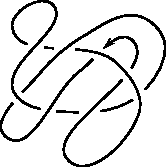
\includegraphics[width=1.5in]{8x_tref.pdf}
%   \end{figure}
% \end{frame}

% \begin{frame}
%   \frametitle{Natural questions about knot diagrams}
%   \begin{block}{Question}
%     What is the average minimal crossing \# of an 8-crossing diagram?\\
%     \onslide<2>{\centering $0.52$}
%   \end{block}
%   \begin{figure}
%     \centering
%     \[
%     \vcenter{\hbox{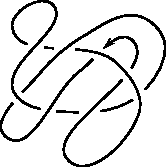
\includegraphics[width=1.5in]{8x_tref.pdf}}}
%     \Rightarrow
%     \vcenter{\hbox{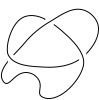
\includegraphics[width=1.5in]{8x_min_tref.pdf}}}
%     \]
%   \end{figure}
% \end{frame}

% \begin{frame}
%   \frametitle{Natural questions about knot diagrams}
%   \begin{definition}
%     The \emph{untwisting} operator deletes all 1-crossing connect
%     summands of a diagram. (Equivalently, performs all ``available''
%     Reidemeister I moves.)
%   \end{definition}

%   \begin{figure}
%     \centering
%     \[
%     \vcenter{\hbox{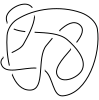
\includegraphics[width=1.5in]{8x_tref_loopy.pdf}}}
%     \Rightarrow
%     \vcenter{\hbox{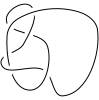
\includegraphics[width=1.5in]{8x_tref_deloopy.pdf}}}
%     \]
%   \end{figure}

% \end{frame}

% \begin{frame}
%   \frametitle{Natural questions about knot diagrams}
%   \begin{block}{Question}
%     What is the average crossing \# of a untwisted 8-crossing diagram?\\
%     \onslide<2>{\centering $2.20$}
%   \end{block}
%   \begin{figure}
%     \centering
%     \[
%     \vcenter{\hbox{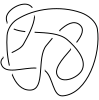
\includegraphics[width=1.5in]{8x_tref_loopy.pdf}}}
%     \Rightarrow
%     \vcenter{\hbox{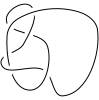
\includegraphics[width=1.5in]{8x_tref_deloopy.pdf}}}
%     \]
%   \end{figure}
% \end{frame}

% \begin{frame}
%   \frametitle{Natural questions about knot diagrams}
%   \begin{block}{Question}
%     How many 8-crossing diagrams can be untwisted to the unknot?\\
%     \onslide<2>{\centering $42.05\%$}
%   \end{block}
%   \begin{figure}
%     \centering
%     \includegraphics[width=1.5in]{tree_like_8x.pdf}
%   \end{figure}
% \end{frame}

\subsection{Background}

\begin{frame}
  %\frametitle{Ansatz}
  \begin{figure}
    \centering
    \begin{tikzpicture}[->,,shorten >=1pt,semithick,align=center]
      % \tikzstyle{every node}=[align=center]
      \node[text width=1in] (plantri)
      {Polymers\\\includegraphics[width=.95in]{dna.jpg}};
      \node[text width=1in,right=.3in of plantri] (isomch)
      {Knots\\\includegraphics[width=.95in]{knot_3d.jpg}};

      \path (plantri) edge (isomch);
    \end{tikzpicture}
  \end{figure}
\end{frame}

\begin{frame}<1>[label=knottheory]
  \frametitle{Knot theory}
  \begin{definition}
    A \emph{knot} is an embedding of the circle $S^1$ into $S^3$, up
    to ambient isotopy. ``String can move but not pass through
    itself.''
  \end{definition}
  \pause
  \begin{theorem}[Reidemeister]
    A \emph{knot} is an equivalence class of \emph{knot diagrams} up
    to changes by the three \emph{Reidemeister moves}.
  \end{theorem}
  \begin{figure}[h!]
  \begin{tabular}{c@{\hspace{2em}}c@{\hspace{2em}}c}
  \centering
  \begin{tikzpicture}[every path/.style={string, very thick}, every node/.style={transform shape,
      knot crossing, inner sep=1.5pt}]
    \begin{scope}
      \node (X) at (0,0) {};
      \node (L) at (0,.7) {};
      \node (lC) at (.5,0) {};

      \node (A) at (-.5,-.5) {};
      \node (B) at (.5,-.5) {};

      \draw (A) -- (X.center);
      \draw (X.center) .. controls (X.4 north east) and (L.4 east) .. (L.center);
      \draw (X) .. controls (X.4 north west) and (L.4 west) .. (L.center);
      \draw (X) -- (B);
    \end{scope}
    \begin{scope}[xshift=.8in]
      \node (A) at (-.5,-.5) {};
      \node (B) at (.5,-.5) {};

      \node (X) at (0,.7) {};
      \node (rC) at (-.5,0) {};

      \draw (A)        .. controls (A.8 north east) and (X.4 west) .. (X.center);
      \draw (X.center) .. controls (X.4 east) and (B.8 north west) .. (B);
    \end{scope}
    \draw[<->] (lC) -- (rC);
  \end{tikzpicture}
    &
  \begin{tikzpicture}[every path/.style={string, very thick}, every node/.style={transform shape,
      knot crossing, inner sep=1.5pt}]
    \begin{scope}
      \node (X1) at (0,-.2) {};
      \node (X2) at (0,.4) {};
      \node (lC) at (.5,0) {};

      \node (A1) at (-.5,-.5) {};
      \node (A2) at (-.5,.7) {};
      \node (B1) at (.5,-.5) {};
      \node (B2) at (.5,.7) {};

      \draw (A1) -- (X1.center);
      \draw (X1.center) .. controls (X1.2 north east) and (X2.2 south east) .. (X2.center);
      \draw (X2.center) -- (A2);

      \draw (B1) -- (X1);
      \draw (X1) .. controls (X1.2 north west) and (X2.2 south west) .. (X2);
      \draw (X2) -- (B2);
    \end{scope}
    \begin{scope}[xshift=.8in]
      \node (A1) at (-.5,-.5) {};
      \node (A2) at (-.5,.7) {};
      \node (B1) at (.5,-.5) {};
      \node (B2) at (.5,.7) {};

      \node (X1) at (-.2,.1) {};
      \node (X2) at (.2,.1) {};
      \node (rC) at (-.5,0) {};

      \draw (A1) .. controls (A1.2 north east) and (X1.2 south) .. (X1.center);
      \draw (A2) .. controls (A2.2 south east) and (X1.2 north) .. (X1.center);
      \draw (B1) .. controls (B1.2 north west) and (X2.2 south) .. (X2.center);
      \draw (B2) .. controls (B2.2 south west) and (X2.2 north) .. (X2.center);
    \end{scope}
    \draw[<->] (lC) -- (rC);
  \end{tikzpicture}
      & \begin{tikzpicture}[every path/.style={string, very thick}, every node/.style={transform shape,
      knot crossing, inner sep=1.5pt}]
    \begin{scope}
      \node (lC) at (.5,0) {};

      \node (A1) at (-.6,-.2) {};
      \node (A2) at (.6,-.2) {};
      \node (B1) at (-.5,-.5) {};
      \node (B2) at (.2,.7) {};
      \node (C1) at (.5,-.5) {};
      \node (C2) at (-.2,.7) {};

      \node (X1) at (-.3,-.2) {};
      \node (X2) at (.3,-.2) {};
      \node (X3) at (0,.3) {};

      \draw (A1) -- (X1.center) -- (X2.center) -- (A2);
      \draw (B1) -- (X1);
      \draw (X1) -- (X3.center) -- (B2);
      \draw (C1) -- (X2) -- (X3) -- (C2);
    \end{scope}
    \begin{scope}[xshift=.8in]
      \node (A1) at (-.6,.4) {};
      \node (A2) at (.6,.4) {};
      \node (B1) at (-.5,.7) {};
      \node (B2) at (.2,-.5) {};
      \node (C1) at (.5,.7) {};
      \node (C2) at (-.2,-.5) {};

      \node (X1) at (-.3,.4) {};
      \node (X2) at (.3,.4) {};
      \node (X3) at (0,-.1) {};

      \draw (A1) -- (X1.center) -- (X2.center) -- (A2);
      \draw (B1) -- (X1);
      \draw (X1) -- (X3) -- (B2);
      \draw (C1) -- (X2) -- (X3.center) -- (C2);

      \node (rC) at (-.5,0) {};
    \end{scope}
    \draw[<->] (lC) -- (rC);
  \end{tikzpicture}

  \end{tabular}
  The three Reidemeister moves.
  \label{fig:reidemeister}
\end{figure}
\end{frame}

\begin{frame}
  %\frametitle{Ansatz}
  \begin{figure}
    \centering
    \begin{tikzpicture}[->,,shorten >=1pt,semithick,align=center]
      % \tikzstyle{every node}=[align=center]
      \node[text width=1in] (plantri)
      {Polymers\\\includegraphics[width=.95in]{dna.jpg}};
      \node[text width=1in,right=.3in of plantri]  (expand)
      {Random curves\\\includegraphics[width=.95in]{space_polygon.jpg}};
      \node[text width=1in,right=.3in of expand] (isomch)
      {Knots\\\includegraphics[width=.95in]{knot_3d.jpg}};

      \path (plantri)    edge (expand)
      (expand)     edge (isomch);
    \end{tikzpicture}
  \end{figure}
\end{frame}

\begin{frame}
  %\frametitle{Combinatorial approaches}
    \begin{figure}
    \centering
    \begin{tikzpicture}[->,,shorten >=1pt,semithick,align=center]
      % \tikzstyle{every node}=[align=center]
      \node[text width=1in] (plantri)
      {Polymers\\\includegraphics[width=.95in]{dna.jpg}};
      \node[text width=1in,right=.3in of plantri]  (expand)
      {Random curves\\\includegraphics[width=.95in]{space_polygon.jpg}};
      \node[text width=1in,right=.3in of expand] (isomch)
      {Knots\\\includegraphics[width=.95in]{knot_3d.jpg}};
      \node[text width=1in,below=.3in of isomch]  (combinatorics)
      {Random combinatorial\\
        \resizebox{.95in}{!}{
          \tikz[thick]{
            \foreach \x in {0,1,...,4} {
              % \draw[white,-,line width = 5] (\x*288-54:3) -- (\x*288+90:3);
              \draw[>=triangle 90 cap,white,<->,line width = 6,shorten >=3, shorten <=3] (\x*288-54:3) -- (\x*288+90:3);
              \draw[black,decoration={markings,mark=at position 0.25 with {\arrow{>}}},postaction={decorate}] (\x*288-54:3) -- (\x*288+90:3); }
            \foreach \x in {0,1,...,4} {
              \draw (\x*144-54:3)+(\x*144+99:1) node[auto,scale=0.7] {\x};}
            %\foreach \p/\x in {24/0,03/1,14/2,02/3,13/4} \node[scale=0.7] at (\x*144-90:1.5){$p_{\p}$};
            %\filldraw (306:3) circle (2pt);
            % \draw[step=0.5,gray,very thin] (-3,-3) grid (3,3);
            \pgfresetboundingbox \clip (-3,-2.75) rectangle (3,3);
          }
        }
      };

      \path (plantri)    edge (expand)
      (expand)     edge (isomch);
      \path (combinatorics) edge (isomch);
    \end{tikzpicture}
  \end{figure}
\end{frame}

\begin{frame}
    \begin{figure}
    \centering
    \begin{tikzpicture}[->,,shorten
      >=1pt,semithick,align=center,minimum height=1.3in]
      % \tikzstyle{every node}=[align=center]
      \node[text width=1in] (plantri)
      {Polymers\\\includegraphics[width=.95in]{dna.jpg}};
      \node[text width=1in,right=.3in of plantri]  (expand)
      {Random curves\\\includegraphics[width=.95in]{space_polygon.jpg}};
      \node[text width=1in,right=.3in of expand] (isomch)
      {Knots\\\includegraphics[width=.95in]{knot_3d.jpg}};
      \node[fill=black,text=white,text width=1in,below=.3in of expand] (diagrams)
      {???};
      \node[text width=1in,below=.3in of isomch]  (combinatorics)
      {Random combinatorial\\
        \resizebox{.95in}{!}{
          \tikz[thick]{
            \foreach \x in {0,1,...,4} {
              % \draw[white,-,line width = 5] (\x*288-54:3) -- (\x*288+90:3);
              \draw[>=triangle 90 cap,white,<->,line width = 6,shorten >=3, shorten <=3] (\x*288-54:3) -- (\x*288+90:3);
              \draw[black,decoration={markings,mark=at position 0.25 with {\arrow{>}}},postaction={decorate}] (\x*288-54:3) -- (\x*288+90:3); }
            \foreach \x in {0,1,...,4} {
              \draw (\x*144-54:3)+(\x*144+99:1) node[auto,scale=0.7] {\x};}
            %\foreach \p/\x in {24/0,03/1,14/2,02/3,13/4} \node[scale=0.7] at (\x*144-90:1.5){$p_{\p}$};
            %\filldraw (306:3) circle (2pt);
            % \draw[step=0.5,gray,very thin] (-3,-3) grid (3,3);
            \pgfresetboundingbox \clip (-3,-2.75) rectangle (3,3);
          }
        }
      };

      \path (plantri)    edge (expand)
      (expand)     edge (isomch);
      \path (combinatorics) edge (isomch);
      \draw[<->] (expand) -- (diagrams);
      \draw[<->] (combinatorics) -- (diagrams);
    \end{tikzpicture}
  \end{figure}

\end{frame}

\againframe{knottheory}

\begin{frame}
  \frametitle{Random diagrams}
  \begin{definition}
    In the \emph{random diagram model} of random knotting, a
    $n$-crossing diagram is drawn uniformly from the finite set of
    $n$-crossing knot diagrams.
  \end{definition}
  \begin{figure}
    \centering
    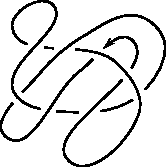
\includegraphics[width=1.2in]{8x_tref.pdf}\qquad
    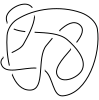
\includegraphics[width=1.2in]{8x_tref_loopy.pdf}\qquad
    \includegraphics[width=1.2in]{tree_like_8x.pdf}
  \end{figure}
  \pause Model is similar to ones considered by Diao-Ernst-Ziegler
  (2004) and Dunfield (2014; in progress)
\end{frame}

\begin{frame}
    \begin{figure}
      \vspace{-.05in}
    \centering
    \begin{tikzpicture}[->,,shorten
      >=1pt,semithick,align=center,minimum height=1.4in]
      % \tikzstyle{every node}=[align=center]
      \node[text width=1in] (plantri)
      {Polymers\\\includegraphics[width=.95in]{dna.jpg}};
      \node[text width=1in,right=.3in of plantri]  (expand)
      {Random curves\\\includegraphics[width=.95in]{space_polygon.jpg}};
      \node[text width=1in,right=.3in of expand] (isomch)
      {Knots\\\includegraphics[width=.95in]{knot_3d.jpg}};
      \node[text width=1in,below=.3in of expand] (diagrams)
      {Random diagrams\\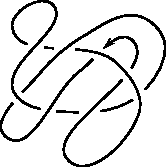
\includegraphics[width=.95in]{8x_tref.pdf}};
      \node[text width=1in,below=.3in of isomch]  (combinatorics)
      {Random combinatorial\\
        \resizebox{.95in}{!}{
          \tikz[thick]{
            \foreach \x in {0,1,...,4} {
              % \draw[white,-,line width = 5] (\x*288-54:3) -- (\x*288+90:3);
              \draw[>=triangle 90 cap,white,<->,line width = 6,shorten >=3, shorten <=3] (\x*288-54:3) -- (\x*288+90:3);
              \draw[black,decoration={markings,mark=at position 0.25 with {\arrow{>}}},postaction={decorate}] (\x*288-54:3) -- (\x*288+90:3); }
            \foreach \x in {0,1,...,4} {
              \draw (\x*144-54:3)+(\x*144+99:1) node[auto,scale=0.7] {\x};}
            %\foreach \p/\x in {24/0,03/1,14/2,02/3,13/4} \node[scale=0.7] at (\x*144-90:1.5){$p_{\p}$};
            %\filldraw (306:3) circle (2pt);
            % \draw[step=0.5,gray,very thin] (-3,-3) grid (3,3);
            \pgfresetboundingbox \clip (-3,-2.75) rectangle (3,3);
          }
        }
      };

      \path (plantri)    edge (expand)
      (expand)     edge (isomch);
      \path (combinatorics) edge (isomch);
      \draw[<->] (expand) -- (diagrams);
      \draw[<->] (combinatorics) -- (diagrams);
      \path (diagrams) edge (isomch);
    \end{tikzpicture}
  \end{figure}

\end{frame}

\begin{frame}
  \frametitle{Knot diagrams}
  \begin{definition}
    A \emph{knot diagram} is a spherically embedded 4-regular graph
    together with extra ``over-under'' information at each vertex.
  \end{definition}
    \begin{figure}
    \centering
    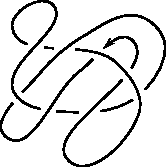
\includegraphics[width=1.2in]{8x_tref.pdf}\qquad
    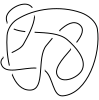
\includegraphics[width=1.2in]{8x_tref_loopy.pdf}\qquad
    \includegraphics[width=1.2in]{tree_like_8x.pdf}
  \end{figure}
  \pause
  \begin{notation}
    A graph embedded on a sphere is called a \emph{planar map}.
  \end{notation}
\end{frame}

\begin{frame}
  \frametitle{The Frisch-Wasserman-Delbr\"uck Conjecture}
  \begin{definition}
    The equivalence class of knots containing the closed trivial loop
    is the \emph{unknot}. A representative of this class is called
    \emph{unknotted}. Otherwise, it is \emph{knotted}.
  \end{definition}
  \pause
  \begin{conjecture}[Frisch-Wasserman 1961, Delbr\"uck 1962]
    The probability that a randomly embedded circle in $\R^3$ is
    knotted tends to one as $n$ tends to infinity.
  \end{conjecture}
  \begin{theorem}[Sumners-Whittington 1988]
    The FWD conjecture holds for $n$-step self avoiding polygons in
    $\R^3$.
  \end{theorem}
  Can prove the conjecture for other space curve models of random
  knotting, too
\end{frame}

\begin{frame}<1>[label=fwddiagrams]
  \frametitle{The Frisch-Wasserman-Delbr\"uck Conjecture}
  Let's reinterpret FWD for our model:
  \begin{conjecture}[Frisch-Wasserman-Delbr\"uck]
    The probability that a knot diagram with $n$ crossings is
    knotted tends to one as $n$ tends to infinity.
  \end{conjecture}
  \pause
  How to prove this? Same idea as Sumners-Whittington's proof!
  \begin{idea}
    Substructure (``patterns'') appear linearly often as the size of
    objects grows.
  \end{idea}
  Then pick patterns that assure knottiness.
\end{frame}

\begin{frame}
  \frametitle{Is this knotted?}

   \begin{center}
     \includegraphics[width=4in]{../figs/random-70cr-1.png}
  \end{center}
\end{frame}

\againframe<2>{fwddiagrams}

\begin{frame}
  \frametitle{Symmetries are tough}
  Symmetries make working with diagrams \emph{difficult}! So kill them...
  \begin{definition}
    A \emph{rooted knot diagram} is a knot diagram together with a
    choice of edge and a choice of direction.
  \end{definition}
    \begin{figure}
    \centering
    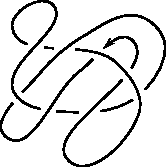
\includegraphics[width=1.2in]{8x_tref.pdf}\qquad
    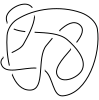
\includegraphics[width=1.2in]{8x_tref_loopy.pdf}\qquad
    \includegraphics[width=1.2in]{tree_like_8x.pdf}
  \end{figure}
  No more nontrivial automorphisms since root must map to itself.
\end{frame}

% \begin{frame}
%   \frametitle{Different diagram classes of interest}
%   We can restrict to different classes of diagrams and prove results
%   for them; some of those considered are,
%   \begin{enumerate}
%   \item \emph{Knot diagrams}: diagrams with precisely one component
%   \item \emph{Link diagrams}: diagrams with any number of
%     components
%   \item \emph{Reduced diagrams}: (knot or link) diagrams which have
%     no disconnecting vertices (called \emph{isthmi})
%   \item \emph{Prime diagrams}: (knot or link) diagrams which cannot
%     be disconnected by removing any pair of edges
%   \end{enumerate}
% \end{frame}


% \begin{frame}
%   \frametitle{Diagram with an isthmus}
%   \begin{figure}[h!]
%     \centering
%     \includegraphics[height=3in]{isthmus.png}
%   \end{figure}
% \end{frame}

% \begin{frame}
%   \frametitle{Prime vs. composite diagrams}
%   \begin{figure}[h!]
%     \centering
%     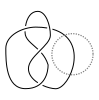
\includegraphics[width=2in]{fig8_triv_tangle.png}
%     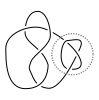
\includegraphics[width=2in]{fig8_subd_tangle.png}
%   \end{figure}
% \end{frame}


% \begin{frame}
%   \frametitle{How to sample diagrams?}
%   \begin{idea}
%     Tabulate all diagrams using software, then draw randomly from the
%     list
%   \end{idea}

%   \begin{caveat}<2-> There are \emph{a lot of} diagrams! 10-crossing
%     link diagrams take 1GB memory; 11-crossing ones take 10GB
%   \end{caveat}

%   \begin{idea}<3->
%     Use clever methods to sample diagrams without total generation
%   \end{idea}

%   % \begin{definition}
%   %   A \emph{knot shadow} is a equivalence class of generic immersions of the unoriented $S^1$
%   %   into the sphere $S^2$ up to diffeomorphism of $S^2$.
%   % \end{definition}

%   % \begin{plan}
%   %  \begin{enumerate}
%   %  \item Enumerate shadows (and discard isomorphic shadows)
%   %  \item Assign crossing and orientation information (and discard crossing patterns related by an automorphism of the shadow)
%   %  \end{enumerate}
%   % \end{plan}

%   \begin{caveat}<4->
%   \emph{Symmetry} makes it difficult to weight probabilities correctly
%   \end{caveat}
% \end{frame}

% \begin{frame}
%   \frametitle{How to sample diagrams}
%   \begin{idea}
%     Efficiently sample \emph{simpler objects} which, in the limit,
%     behave like diagrams
%   \end{idea}

%   This will work!

%   \begin{definition}<2->
%     A \emph{rooted diagram} is a diagram together with a choice of
%     edge, called the \emph{root edge} and a direction for that edge
%   \end{definition}

%   \begin{theorem}[C.]<2-> The ratio of diagrams with $n$ crossings
%     which have nontrivial automorphism group is exponentially
%     small. Hence asymptotically, rooted diagrams behave like diagrams.
%   \end{theorem}

% \end{frame}

\begin{frame}
   \frametitle{...Is that really okay?}

   \begin{center}
   \includegraphics[width=4in]{../figs/mean-automorphisms.pdf}
   \end{center}

\end{frame}

\begin{frame}
  \frametitle{Patterns du jour}
  \begin{definition}
    \begin{itemize}
    \item A \emph{$2k$-tangle} is a diagram-like object having $2k$
      half-edges which lie in the exterior face.

    \item A tangle is contained in a diagram $D$ if there exists some disk
      which, when intersected with $D$, produces the tangle.
    \end{itemize}
  \end{definition}
  \begin{figure}[h!]
    \centering
    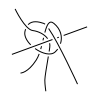
\includegraphics[height=1.5in]{6-tangle.pdf}
    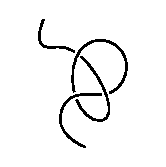
\includegraphics[height=1.5in]{silly_2tangle.pdf}
    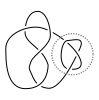
\includegraphics[height=1.3in]{fig8_subd_tangle.pdf}
  \end{figure}
\end{frame}

% \begin{frame}
%   \frametitle{Rooted diagrams and 2-tangles}
%   Rooted (knot or link) diagrams are equivalently viewed as
%   \emph{2-tangles}
% \begin{figure}[h!]  \centering
%   \begin{tikzpicture}[scale=.8,every path/.style={string, very thick}, every node/.style={transform shape,
%       knot crossing, inner sep=1.5pt}]
%     \begin{scope}[xshift=-1.5in] \node (tl) at (-.7,0) {}; \node (tr)
%       at (.7,0) {}; \node (tc) at (0,1) {}; \draw (tl) .. controls (tl.4
%       north east) and (tc.4 south west) ..  (tc.center); \draw (tc.center)
%       .. controls (tc.8 north east) and (tr.8 north east) .. (tr); \draw
%       (tr) .. controls (tr.4 south west) and (tl.4 south east)
%       .. (tl.center); \draw (tl.center) .. controls (tl.8 north west) and
%       (tc.8 north west) .. (tc); \draw (tc) .. controls (tc.4 south east)
%       and (tr.4 north west) .. (tr.center); \draw[->=.5] (tr.center)
%       .. controls (tr.16 south east) and (tl.16 south west) .. (tl);
%     \end{scope}

%     \begin{scope}[xshift=1.5in] \node (tl) at (-.7,0) {}; \node (tr)
%       at (.7,0) {}; \node (tc) at (0,1) {}; \node (el) at (-1.7,0) {}; \node
%       (er) at (1.7,0) {}; \draw[>-] (el.center) .. controls (el.4 east) and
%       (tl.4 south west) .. (tl); \draw (tl) .. controls (tl.4 north east)
%       and (tc.4 south west) ..  (tc.center); \draw (tc.center) .. controls
%       (tc.8 north east) and (tr.8 north east) .. (tr); \draw (tr)
%       .. controls (tr.4 south west) and (tl.4 south east) .. (tl.center);
%       \draw (tl.center) .. controls (tl.8 north west) and (tc.8 north west)
%       .. (tc); \draw (tc) .. controls (tc.4 south east) and (tr.4 north
%       west) .. (tr.center); \draw[->] (tr.center) .. controls (tr.4 south
%       east) and (er.4 west) .. (er.center);
%     \end{scope} \draw[<->] (-1.6,.3) -- (1,.3) node[text
%     width=3cm,text centered,midway]{cut/splice root edge};
%   \end{tikzpicture}
%   %\caption{Rooted diagrams of the trefoil and its mirror image}
%   \label{fig:treflegs2}
% \end{figure}

% \end{frame}

\begin{frame}
  \frametitle{A pattern theorem for knot diagrams}
  Indeed (adapting a proof of Bender-Gao-Richmond 1992),
  \begin{theorem}[C.]
    Let $\KnotDia$ be the class of rooted knot diagrams and
    $\KnotDia_n$ be the set of rooted knot diagrams with $n$
    crossings. Let $P$ be a tangle which is appropriately
    ``admissible.'' Then there exist constants $c > 0$ and $d < 1$ so
    that
    \[ \Prb(\text{$D$ in $\KnotDia_n$ contains $\le cn$
      copies of $P$ as a subtangle}) < d^n.\]
  \end{theorem}
  \pause
  \begin{proof}[Key requirement for proof]
    There is an ``attachment'' operation on diagrams which
    produces a new diagram containing $P$ so that for some $k$
    depending on the attachment, a diagram in $n$ crossings has $n/k$
    valid attachment sites.
  \end{proof}
\end{frame}

\begin{frame}
  \frametitle{Admissible tangles}
  Knot diagrams and any 2-tangle of one component; expansion
  operation: connect summation
  \begin{figure}[h!]
    \centering
    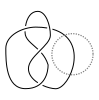
\includegraphics[height=1.3in]{fig8_triv_tangle.pdf}
    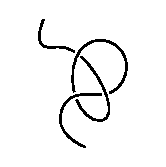
\includegraphics[height=1.3in]{silly_2tangle.pdf}
    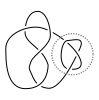
\includegraphics[height=1.3in]{fig8_subd_tangle.pdf}
  \end{figure}
\end{frame}

\begin{frame}
  \frametitle{Admissible tangles}
  Knot diagrams and any $2k$-tangle of $k$ components; expansion
  operation: connect summation (after placing into a 2-tangle)
  \begin{figure}[h!]
    \centering
    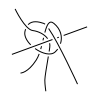
\includegraphics[height=1.3in]{6-tangle.pdf}
    \includegraphics[height=1.3in]{6tangle-as-2tangle.pdf}
  \end{figure}
\end{frame}

% \begin{frame}
%   \frametitle{Admissible tangles}
%   Knot diagrams (prime, reduced, or otherwise) and any prime $abab$
%   $4$-tangle of two components; expansion operation: 4-tangle
%   replacement
%   \begin{figure}[h!]
%     \centering
%     \includegraphics[height=1.3in]{tref_triv_tangle.png}
%     \includegraphics[height=1.3in]{abab_tangle.png}
%     \includegraphics[height=1.3in]{tref_subd_tangle.png}
%   \end{figure}
% \end{frame}

\begin{frame}
  \frametitle{A technical lemma}
  \begin{caveat}
    It's actually required in the proof of the pattern theorem that
    $\KnotDia$ grows \emph{smoothly}; that
    \[ \lim_{n \to \infty}{|\KnotDia_n|^{1/n}} = \limsup_{n \to
      \infty}{|\KnotDia_n|^{1/n}}.\]
  \end{caveat}
  \only<2>{Asymptotics of knot diagrams are wholly unknown! There are only
    conjectures...
    \begin{conjecture}[Schaeffer-P. Zinn-Justin 2004]
      The number of rooted knot diagrams grows like
      \[ |\KnotDia_n| \mathop{\sim}\limits_{n\to\infty}
      c\tau^nn^{\gamma-2}, \quad \text{where }\gamma = -\frac{1 +
        \sqrt{13}}{6} \approx -0.76759... \]
    \end{conjecture}}
  \only<3>{Fortunately (using methods of BGR 1992),
    \begin{lemma}[C.]
      The class of rooted knot diagrams grow smoothly.
    \end{lemma}}
\end{frame}


% \begin{frame}
%   \frametitle{Smooth growth for diagrams}

%   \begin{proof}[Idea of proof]
%     \begin{enumerate}
%     \item Let $\KnotDia$ be the class of interest
%     \item We know
%       $\limsup_{n\to\infty}{|\KnotDia_n|}^{1/n}$ exists
%       (Cauchy-Hadamard), so there exists $n$ where there are ``enough''
%       diagrams in $\KnotDia_n$
%     \item Find $m > n$ and injections from $\KnotDia_n$ into
%       $\KnotDia_m$ and $\KnotDia_{m+1}$
%     \item Define a ``nice'' composition on diagrams to get lower
%       bounds on $|\KnotDia_N|$ for large $N$ and, hence, $\liminf_{n\to\infty}{|\KnotDia_n|}^{1/n}$ \qedhere
%     \end{enumerate}
%   \end{proof}

% \end{frame}

\tikzset{global scale/.style={
    scale=#1,
    every node/.style={scale=#1}
  }
}

\begin{frame}
  \frametitle{Smooth growth for knot diagrams}
  \begin{proof}[(Very!) Rough idea of proof]
    \begin{itemize}[<+->]
    \item It's possible to make $(n+1)$-crossing diagrams from $n$-crossing diagrams
      \vspace{-.7cm}
      \begin{figure}[h!]  \centering
        \[
        \begin{aligned}
          \begin{tikzpicture}[global scale=.7,every path/.style={very
              thick},decoration={markings, mark=at position 0.5 with
              {\arrow{>}}}]
            \node[draw,circle,minimum size=15pt] (A) at (0,0) {$K_1$};
            \node[draw,circle,minimum size=15pt] (B) at (1,0) {$K_2$};
            \node[draw,circle,minimum size=15pt] (C) at (2.5,0) {$K_\ell$};
            \node (L) at (0,-.8) {};
            \node (R) at (2.5,-.8) {};

            \draw (L.center) -- (A);
            \draw (A) -- (B);
            \draw[dotted] (B) -- (C);
            \draw (C) -- (R.center);
            \draw (R.center) edge[out=-90,in=-90,postaction={decorate}] (L.center);
          \end{tikzpicture}
        \end{aligned} \xmapsto{\varphi}
        \begin{aligned}
          \begin{tikzpicture}[global scale=.7,every path/.style={very
              thick},decoration={markings, mark=at position 0.5 with
              {\arrow{>}}}]
            \node[draw,circle,minimum size=15pt] (A) at (0,0) {$K_1$};
            \node[draw,circle,minimum size=15pt] (B) at (1,0) {$K_2$};
            \node[draw,circle,minimum size=15pt] (C) at (2.5,0) {$K_\ell$};
            \node[draw,circle,fill=black,inner sep=2pt] (X) at (1.25,-1) {};

            \draw (X) edge[in=-70,out=90+45] (A);
            \draw (A) -- (B);
            \draw[dotted] (B) -- (C);
            \draw (C) edge[out=-110,in=90-45] (X);
            \draw (X) edge[out=-135,in=-45,postaction={decorate},looseness=10] (X);
          \end{tikzpicture}
        \end{aligned} \xmapsto{\varphi}
        \begin{aligned}
          \begin{tikzpicture}[global scale=.7,every path/.style={very
              thick},decoration={markings, mark=at position 0.5 with
              {\arrow{>}}}]
            \node[draw,circle,minimum size=15pt] (A) at (0,0) {$K_1$};
            \node[draw,circle,minimum size=15pt] (B) at (1,0) {$K_2$};
            \node[draw,circle,minimum size=15pt] (C) at (2.5,0) {$K_\ell$};
            \node[draw,circle,fill=black,inner sep=2pt] (X) at (1.25,-1) {};
            \node[draw,circle,fill=black,inner sep=2pt] (Y) at (1.25,-1.8) {};

            \draw (X) edge[in=-70,out=90+45] (A);
            \draw (A) -- (B);
            \draw[dotted] (B) -- (C);
            \draw (C) edge[out=-110,in=90-45] (X);
            \draw (X) edge[bend right] (Y);
            \draw (X) edge[bend left] (Y);
            \draw (Y) edge[out=-45,in=-135,postaction={decorate},looseness=10] (Y);
          \end{tikzpicture}
        \end{aligned}
        \]
        \label{fig:phi_e xample}
      \end{figure}
      \vspace{-.7cm}
    \item And it's possible to create $(n+m)$-crossing diagrams from
      $n$-crossing diagrams and $m$-crossing diagrams.\vspace{-.5cm}
      \begin{figure}[h!]  \centering
        \[
        \begin{aligned}
          \begin{tikzpicture}[global scale=.7,every path/.style={very
              thick}]
            \node[draw,circle,minimum size=40pt] (A) at (0,0) {$K_1$};
            \node (L) at (-1.5,0) {};
            \node (R) at (1.5,0) {};

            \draw[>-] (L.center) -- (A);
            \draw[->] (A) -- (R.center);
          \end{tikzpicture}
        \end{aligned} \#
        \begin{aligned}
          \begin{tikzpicture}[global scale=.7,every path/.style={very
              thick}]
            \node[draw,circle,minimum size=40pt] (A) at (0,0) {$K_2$};
            \node (L) at (-1.5,0) {};
            \node (R) at (1.5,0) {};

            \draw[>-] (L.center) -- (A);
            \draw[->] (A) -- (R.center);
          \end{tikzpicture}
        \end{aligned} =
        \begin{aligned}
          \begin{tikzpicture}[global scale=.7,every path/.style={very
              thick}]
            \node[draw,circle,minimum size=40pt] (A) at (0,0) {$K_1$};
            \node[draw,circle,minimum size=40pt] (B) at (2,0) {$K_2$};
            \node (L) at (-1.5,0) {};
            \node (R) at (3.5,0) {};

            \draw[>-] (L.center) -- (A);
            \draw (A) -- (B);
            \draw[->] (B) -- (R.center);
          \end{tikzpicture}
        \end{aligned}
        \]
        \label{fig:legsum_example}
      \end{figure}

    \end{itemize}
  \end{proof}
\end{frame}

\begin{frame}
   \frametitle{Remember this?}

   \begin{center}
   \includegraphics[width=4in]{../figs/mean-automorphisms.pdf}
   \end{center}
\end{frame}

\begin{frame}
  \frametitle{Asymmetry of knot diagrams}
  The pattern theorem comes with a handy bonus (together with a
  theorem of Richmond-Wormald 1995):
  \begin{theorem}[C.]
    Almost all unrooted knot diagrams have only trivial
    automorphism group.
  \end{theorem}
  So for large $n$, rooted knot diagrams map
  $4n$-to-one to unrooted knot diagrams.\pause ~Hence;
  \begin{corollary}[C.]
    Unrooted knot diagrams have the pattern theorem
  \end{corollary}
  \pause
  \begin{corollary}[C.]
    Unrooted knot diagrams are almost certainly knotted
  \end{corollary}
\end{frame}

\begin{frame}
  \frametitle{Recap from work with Cantarella and Mastin}
  \begin{idea}[Cantarella-C.-Mastin]
    Sample from the random (unrooted) knot diagram model via complete
    enumeration. (No other obvious methods)
  \end{idea}
  \pause
  \begin{problem}
    There are \emph{way} too many knot diagrams. Too many even for 11 crossings!
  \end{problem}
  \pause
  \begin{idea}
    We can closely approximate the random unrooted diagram model by
    the random rooted diagram model. So just sample from the rooted
    diagram model.
  \end{idea}
\end{frame}

\begin{frame}
  \frametitle{The game plan}
    \begin{fact}
    \begin{itemize}[<+->]
    \item Can sample rooted 4-regular planar maps in $O(n)$ (Schaeffer 2003) [Great!]
    \item Can sample $n$ crossing signs uniformly, quickly [Excellent!]
    \item Knot diagrams become asymptotically rare! [Rats!]
    \item \emph{However}, we can still improve on CCM about ten-fold! [Whew...]
    \end{itemize}
  \end{fact}
\end{frame}

\begin{frame}
   \begin{center}
    \only<1>{\includegraphics[width=4in]{../figs/random-70cr-1.png}}
    \only<2>{\includegraphics[height=3in]{../figs/random-70cr-2.png}}
    \only<3>{\includegraphics[height=3in]{../figs/random-70cr-3.png}}
   \end{center}
\end{frame}

\begin{frame}
  \frametitle{The first few knot types}
  \vfill
  \begin{center}
    \includegraphics[width=4in]{knottypes.png}
  \end{center}
  %\vfill
\end{frame}

\begin{frame}
  \begin{figure}
    \centering
    \begin{tikzpicture}[every axis plot/.append style={line width=2pt}]
      \begin{axis}[
        %ymode=log,
        %log ticks with fixed point,
        title={(Exact) ratios of knots in $n$-crossing diagrams},
        xlabel={\# crossings in diagram},
        ylabel={ratios of knots},
        cycle list name=Set1-9,
        legend pos=outer north east,
        legend entries={$3_1$, $4_1$, $5_1$, $5_2$, $0_1$},
        xmax=9,
        ymin=0, ymax=0.15,
        ]
        \addplot table[x=n,y expr=\thisrow{3.1}*2] {knot_freq.tsv};
        \addplot table[x=n,y=4.1] {knot_freq.tsv};
        \addplot table[x=n,y expr=\thisrow{5.1}*2] {knot_freq.tsv};
        \addplot table[x=n,y=5.2] {knot_freq.tsv};
      \end{axis}
    \end{tikzpicture}
    \label{fig:kgrow1}
  \end{figure}
\end{frame}

\begin{frame}
  \begin{figure}
    \centering
    \begin{tikzpicture}[%scale=1,
      every axis plot/.append style={line width=2pt}]
      \begin{axis}[
        %ymode=log,
        %log ticks with fixed point,
        title={(Experimental) ratios of knots in $n$-crossing (rooted) diagrams},
        xlabel={\# crossings in diagram},
        ylabel={ratios of knots},
        cycle list name=Set1-9,
        legend pos=outer north east,
        legend entries={$3_1$, $4_1$, $5_1$, $5_2$, $3_1\#3_1$, $3_1\#3_1^*$},
        xmax=9,
        ymin=0, ymax=0.15,
        ]
        \addplot table[x=n,y expr=\thisrow{3.1}/\thisrow{total}] {sample.tsv};
        \addplot table[x=n,y expr=\thisrow{4.1}/\thisrow{total}] {sample.tsv};
        \addplot table[x=n,y expr=\thisrow{5.1}/\thisrow{total}] {sample.tsv};
        \addplot table[x=n,y expr=\thisrow{5.2}/\thisrow{total}] {sample.tsv};
      \end{axis}
    \end{tikzpicture}
    \label{fig:kgrow1}
  \end{figure}
\end{frame}

\begin{frame}
  \frametitle{Let's throw in some composite knots}
  \vfill
  \begin{center}
    \includegraphics[width=1.6in]{granny.png}

    \includegraphics[width=1.6in]{square.png}
    \\
    {Granny knot $3_1\#3_1$ (top) vs square knot $3_1\#3_1^*$ (bottom)}
  \end{center}
  %\vfill
\end{frame}

\begin{frame}
  \begin{figure}
    \centering
    \begin{tikzpicture}[%scale=1,
      every axis plot/.append style={line width=2pt}]
      \begin{axis}[
        %ymode=log,
        %log ticks with fixed point,
        title={Ratios of knots in $n$-crossing diagrams},
        xlabel={\# crossings in diagram},
        ylabel={ratios of knots},
        cycle list name=Set1-7,
        legend pos=outer north east,
        legend entries={$3_1$, $4_1$, $5_1$, $5_2$, $3_1\#3_1$, $3_1\#3_1^*$, $0_1$},
        xmin=0, xmax=70,
        ymin=0, ymax=1,
        ]
        \addplot table[x=n,y expr=\thisrow{3.1}/\thisrow{total}] {sample.tsv};
        \addplot table[x=n,y expr=\thisrow{4.1}/\thisrow{total}] {sample.tsv};
        \addplot table[x=n,y expr=\thisrow{5.1}/\thisrow{total}] {sample.tsv};
        \addplot table[x=n,y expr=\thisrow{5.2}/\thisrow{total}] {sample.tsv};
        \addplot table[x=n,y expr=\thisrow{3.1c3.1}/\thisrow{total}] {sample.tsv};
        \addplot table[x=n,y expr=\thisrow{3.1c3.1m}/\thisrow{total}] {sample.tsv};
        \addplot table[x=n,y expr=\thisrow{0.1}/\thisrow{total}] {sample.tsv};
      \end{axis}
    \end{tikzpicture}
    \label{fig:kgrow1}
  \end{figure}
\end{frame}

\begin{frame}
  \begin{figure}
    \centering
    \begin{tikzpicture}[%scale=1,
      every axis plot/.append style={line width=2pt}]
      \begin{axis}[
        %ymode=log,
        %log ticks with fixed point,
        title={Ratios of knots in $n$-crossing diagrams},
        xlabel={\# crossings in diagram},
        ylabel={ratios of knots},
        cycle list name=Set1-7,
        legend pos=outer north east,
        legend entries={$3_1$, $4_1$, $5_1$, $5_2$, $3_1\#3_1$, $3_1\#3_1^*$, $0_1$},
        xmin=0, xmax=70,
        ymin=0, ymax=0.1,
        ]
        \addplot table[x=n,y expr=\thisrow{3.1}/\thisrow{total}] {sample.tsv};
        \addplot table[x=n,y expr=\thisrow{4.1}/\thisrow{total}] {sample.tsv};
        \addplot table[x=n,y expr=\thisrow{5.1}/\thisrow{total}] {sample.tsv};
        \addplot table[x=n,y expr=\thisrow{5.2}/\thisrow{total}] {sample.tsv};
        \addplot table[x=n,y expr=\thisrow{3.1c3.1}/\thisrow{total}] {sample.tsv};
        \addplot table[x=n,y expr=\thisrow{3.1c3.1m}/\thisrow{total}] {sample.tsv};
        \addplot table[x=n,y expr=\thisrow{0.1}/\thisrow{total}] {sample.tsv};
      \end{axis}
    \end{tikzpicture}
    \label{fig:kgrow1}
  \end{figure}
\end{frame}

\begin{frame}
  \begin{figure}
    \centering
    \begin{tikzpicture}[%scale=1,
      every axis plot/.append style={line width=2pt}]
      \begin{axis}[
        ymode=log,
        log ticks with fixed point,
        title={Ratios of knots in $n$-crossing diagrams (log plot)},
        xlabel={\# crossings in diagram},
        ylabel={log(ratios of knots)},
        cycle list name=Set1-7,
        legend pos=outer north east,
        legend entries={$3_1$, $4_1$, $5_1$, $5_2$, $3_1\#3_1$, $3_1\#3_1^*$, $0_1$},
        xmin=0, xmax=70,
        ymin=0, ymax=1,
        ]
        \addplot table[x=n,y expr=\thisrow{3.1}/\thisrow{total}] {sample.tsv};
        \addplot table[x=n,y expr=\thisrow{4.1}/\thisrow{total}] {sample.tsv};
        \addplot table[x=n,y expr=\thisrow{5.1}/\thisrow{total}] {sample.tsv};
        \addplot table[x=n,y expr=\thisrow{5.2}/\thisrow{total}] {sample.tsv};
        \addplot table[x=n,y expr=\thisrow{3.1c3.1}/\thisrow{total}] {sample.tsv};
        \addplot table[x=n,y expr=\thisrow{3.1c3.1m}/\thisrow{total}] {sample.tsv};
        \addplot table[x=n,y expr=\thisrow{0.1}/\thisrow{total}] {sample.tsv};
      \end{axis}
    \end{tikzpicture}
    \label{fig:kgrow1}
  \end{figure}
\end{frame}

% \begin{frame}
%   \begin{figure}
%     \centering
%     \begin{tikzpicture}[%scale=1,
%       every axis plot/.append style={line width=2pt}]
%       \begin{axis}[
%         title={Ratios of knots in $n$-crossing diagrams (growth rate)},
%         xlabel={\# crossings in diagram},
%         ylabel={log(ratios of knots)},
%         cycle list name=Set1-7,
%         legend pos=outer north east,
%         legend entries={$3_1$, $4_1$, $5_1$, $5_2$, $3_1\#3_1$, $3_1\#3_1^*$, $0_1$},
%         xmin=60, xmax=70,
%         %ymin=0, ymax=.2,
%         ]
%         \addplot table[x=n,y expr=ln(\thisrow{3.1}/\thisrow{total})/x] {sample.tsv};
%         \addplot table[x=n,y expr=ln(\thisrow{4.1}/\thisrow{total})/x] {sample.tsv};
%         \addplot table[x=n,y expr=ln(\thisrow{5.1}/\thisrow{total})/x] {sample.tsv};
%         \addplot table[x=n,y expr=ln(\thisrow{5.2}/\thisrow{total})/x] {sample.tsv};
%         \addplot table[x=n,y expr=ln(\thisrow{3.1c3.1}/\thisrow{total})/x] {sample.tsv};
%         \addplot table[x=n,y expr=ln(\thisrow{3.1c3.1m}/\thisrow{total})/x] {sample.tsv};
%         \addplot table[x=n,y expr=ln(\thisrow{0.1}/\thisrow{total})/x] {sample.tsv};
%       \end{axis}
%     \end{tikzpicture}
%     \label{fig:kgrow1}
%   \end{figure}
% \end{frame}


%%%%
\makeatletter
\def\pgfplots@getautoplotspec into#1{%
    \begingroup
    \let#1=\pgfutil@empty
    \pgfkeysgetvalue{/pgfplots/cycle multi list/@dim}\pgfplots@cycle@dim
    %
    \let\pgfplots@listindex=\pgfplots@numplots
    %%% Start new code
    \pgfkeysgetvalue{/pgfplots/cycle list set}\pgfplots@listindex@set
    \ifx\pgfplots@listindex@set\pgfutil@empty
    \else
        \c@pgf@counta=\pgfplots@listindex
        \c@pgf@countb=\pgfplots@listindex@set
        \advance\c@pgf@countb by -\c@pgf@counta
        \globaldefs=1\relax
        \edef\setshift{%
            \noexpand\pgfkeys{
                /pgfplots/cycle list shift=\the\c@pgf@countb,
                /pgfplots/cycle list set=
            }
        }%
        \setshift%
    \fi
    %%% End new code
    \pgfkeysgetvalue{/pgfplots/cycle list shift}\pgfplots@listindex@shift
    \ifx\pgfplots@listindex@shift\pgfutil@empty
    \else
        \c@pgf@counta=\pgfplots@listindex\relax
        \advance\c@pgf@counta by\pgfplots@listindex@shift\relax
        \ifnum\c@pgf@counta<0
            \c@pgf@counta=-\c@pgf@counta
        \fi
        \edef\pgfplots@listindex{\the\c@pgf@counta}%
    \fi
    \ifnum\pgfplots@cycle@dim>0
        % use the 'cycle multi list' feature.
        %
        % it employs a scalar -> multiindex map like
        % void fromScalar( size_t d, size_t scalar, size_t* Iout, const size_t* N )
        % {
        %   size_t ret=scalar;
        %   for( int i = d-1; i>=0; --i ) {
        %       Iout[i] = ret % N[i];
        %       ret /= N[i];
        %   }
        % }
        % to get the different indices into the cycle lists.
        %--------------------------------------------------
        \c@pgf@counta=\pgfplots@cycle@dim\relax
        \c@pgf@countb=\pgfplots@listindex\relax
        \advance\c@pgf@counta by-1
        \pgfplotsloop{%
            \ifnum\c@pgf@counta<0
                \pgfplotsloopcontinuefalse
            \else
                \pgfplotsloopcontinuetrue
            \fi
        }{%
            \pgfkeysgetvalue{/pgfplots/cycle multi list/@N\the\c@pgf@counta}\pgfplots@cycle@N
            % compute list index:
            \pgfplotsmathmodint{\c@pgf@countb}{\pgfplots@cycle@N}%
            \divide\c@pgf@countb by \pgfplots@cycle@N\relax
            %
            \expandafter\pgfplots@getautoplotspec@
                \csname pgfp@cyclist@/pgfplots/cycle multi list/@list\the\c@pgf@counta @\endcsname
                {\pgfplots@cycle@N}%
                {\pgfmathresult}%
            \t@pgfplots@toka=\expandafter{#1,}%
            \t@pgfplots@tokb=\expandafter{\pgfplotsretval}%
            \edef#1{\the\t@pgfplots@toka\the\t@pgfplots@tokb}%
            \advance\c@pgf@counta by-1
        }%
    \else
        % normal cycle list:
        \pgfplotslistsize\autoplotspeclist\to\c@pgf@countd
        \pgfplots@getautoplotspec@{\autoplotspeclist}{\c@pgf@countd}{\pgfplots@listindex}%
        \let#1=\pgfplotsretval
    \fi
    \pgfmath@smuggleone#1%
    \endgroup
}

\pgfplotsset{
    cycle list set/.initial=
}
\makeatother
%%%%


\begin{frame}
  \begin{figure}
    \centering
    \begin{tikzpicture}[%scale=1,
      every axis plot/.append style={line width=2pt}]
      \begin{axis}[
        %ymode=log,
        %log ticks with fixed point,
        stack plots=y,
        title={Ratios of knots in $n$-crossing diagrams (stacked)},
        xlabel={\# crossings in diagram},
        ylabel={ratios of knots},
        cycle list name=Set1-7,
        legend pos=outer north east,
        legend entries={$0_1$, $3_1$, $4_1$, $5_1$, $5_2$, $3_1\#3_1$, $3_1\#3_1^*$},
        xmin=0, xmax=70,
        ymin=0, ymax=1,
        ]
        \pgfplotsset{cycle list set=6}
        \addplot table[x=n,y expr=\thisrow{0.1}/\thisrow{total}] {sample.tsv};
        \pgfplotsset{cycle list set=0}
        \addplot table[x=n,y expr=\thisrow{3.1}/\thisrow{total}] {sample.tsv};
        \addplot table[x=n,y expr=\thisrow{4.1}/\thisrow{total}] {sample.tsv};
        \addplot table[x=n,y expr=\thisrow{5.1}/\thisrow{total}] {sample.tsv};
        \addplot table[x=n,y expr=\thisrow{5.2}/\thisrow{total}] {sample.tsv};
        \addplot table[x=n,y expr=\thisrow{3.1c3.1}/\thisrow{total}] {sample.tsv};
        \addplot table[x=n,y expr=\thisrow{3.1c3.1m}/\thisrow{total}] {sample.tsv};
      \end{axis}
    \end{tikzpicture}
    \label{fig:kgrow1}
  \end{figure}
\end{frame}

\begin{frame}
  \begin{figure}
    \centering
    \begin{tikzpicture}[%scale=1,
      every axis plot/.append style={line width=2pt}]
      \begin{axis}[
        %ymode=log,
        %log ticks with fixed point,
        title={Average Vassiliev-2 invariant for $n$ crossing immersions $S^1 \hookrightarrow S^3$},
        xlabel={\# crossings in diagram},
        ylabel={average $v_2^{avg}$},
        cycle list name=Set1-7,
        legend pos=outer north east,
        legend entries={$v_2^{avg}$},
        xmin=0, xmax=70,
        ymin=0, ymax=8,
        ]
        \addplot table[x=n,y expr=\thisrow{v2}] {sample.tsv};
      \end{axis}
    \end{tikzpicture}
    \label{fig:kgrow1}
  \end{figure}
\end{frame}

% \begin{frame}
%   \frametitle{Knotting in diagrams; tabulation data}
%   \begin{figure}
%     \centering
%       \tikzset{mark=*}
%     \begin{tikzpicture}[scale=1]
%       \begin{axis}[
%         ymode=log,
%         log ticks with fixed point,
%         title={Ratios of knots in $n$-crossing diagrams (log scale)},
%         xlabel={\# crossings in diagram},
%         ylabel={Ratios of knots},
%         cycle list name=Mark-Set1-9,
%         legend style={font=\tiny},
%         legend pos=outer north east,
%         legend entries={$3_1$, $4_1$, $5_1$, $5_2$, $6_1$, $6_2$, $3_1
%           \# 3_1$, $3_1 \# 3_1^*$, $7_1$, $7_2$, $7_3$, $7_4$, $7_5$,
%           $7_6$, $7_7$},
%         ]
%         \addplot table[x=n,y=3.1] {knot_freq.tsv};
%         \addplot table[x=n,y=4.1] {knot_freq.tsv};
%         \addplot table[x=n,y=5.1] {knot_freq.tsv};
%         \addplot table[x=n,y=5.2] {knot_freq.tsv};
%         \addplot table[x=n,y=6.1] {knot_freq.tsv};
%         \addplot table[x=n,y=6.2] {knot_freq.tsv};
%         \addplot table[x=n,y=3.1c3.1] {knot_freq.tsv};
%         \addplot table[x=n,y=3.1c3.1m] {knot_freq.tsv};
%         \addplot table[x=n,y=7.1] {knot_freq.tsv};
%         \addplot table[x=n,y=7.2] {knot_freq.tsv};
%         \addplot table[x=n,y=7.3] {knot_freq.tsv};
%         \addplot table[x=n,y=7.4] {knot_freq.tsv};
%         \addplot table[x=n,y=7.5] {knot_freq.tsv};
%         \addplot table[x=n,y=7.6] {knot_freq.tsv};
%         \addplot table[x=n,y=7.7] {knot_freq.tsv};
%       \end{axis}
%     \end{tikzpicture}

%     \label{fig:kgrow2}
%   \end{figure}
% \end{frame}


% \begin{frame}
%   \frametitle{Knotting in diagrams; random sampling}
%   \begin{figure}
%     \centering
%     \begin{tikzpicture}[scale=1]
%       \begin{axis}[
%         %ymode=log,
%         %log ticks with fixed point,
%         title={Ratios of knots in $n$-crossing diagrams},
%         xlabel={\# crossings in diagram},
%         ylabel={Ratios of knots},
%         cycle list name=Dark2-8,
%         legend pos=outer north east,
%         legend entries={$3_1$, $4_1$, $5_1$, $5_2$, $3_1\#3_1$, $3_1\#3_1^*$, $0_1$},
%         ymin=0, ymax=1,
%         ]
%         \addplot table[x=n,y=3.1] {samp_knot_probs.tsv};
%         \addplot table[x=n,y=4.1] {samp_knot_probs.tsv};
%         \addplot table[x=n,y=5.1] {samp_knot_probs.tsv};
%         \addplot table[x=n,y=5.2] {samp_knot_probs.tsv};
%         \addplot table[x=n,y=3.1c3.1] {samp_knot_probs.tsv};
%         \addplot table[x=n,y=3.1c3.1m] {samp_knot_probs.tsv};
%         \addplot table[x=n,y=0.1] {samp_knot_probs.tsv};
%       \end{axis}
%     \end{tikzpicture}
%     \label{fig:kgrow1}
%   \end{figure}
% \end{frame}


% \begin{frame}
%   \frametitle{Knotting in diagrams; random sampling}
%   \begin{figure}
%     \centering
%     \begin{tikzpicture}[scale=1]
%       \begin{axis}[
%         ymode=log,
%         log ticks with fixed point,
%         title={Ratios of knots in $n$-crossing diagrams (log scale)},
%         xlabel={\# crossings in diagram},
%         ylabel={Ratios of knots},
%         cycle list name=Dark2-8,
%         legend pos=outer north east,
%         legend entries={$3_1$, $4_1$, $5_1$, $5_2$, $3_1\#3_1$, $3_1\#3_1^*$},
%         ]
%         \addplot table[x=n,y=3.1] {samp_knot_probs.tsv};
%         \addplot table[x=n,y=4.1] {samp_knot_probs.tsv};
%         \addplot table[x=n,y=5.1] {samp_knot_probs.tsv};
%         \addplot table[x=n,y=5.2] {samp_knot_probs.tsv};
%         \addplot table[x=n,y=3.1c3.1] {samp_knot_probs.tsv};
%         \addplot table[x=n,y=3.1c3.1m] {samp_knot_probs.tsv};
%       \end{axis}
%     \end{tikzpicture}
%     \label{fig:kgrow1}
%   \end{figure}
% \end{frame}


% % \begin{frame}
% %   \frametitle{Duals to quadrangulations}
% %   \begin{figure}
% %     \hphantom{.}
% %     \hfill
% %     \includegraphics[height=1.25in]{quadrangulation} \hfill
% %     \includegraphics[height=1.25in]{non-simple-quadrangulation}
% %     \hfill
% %     \hphantom{.}
% %     \caption{\label{fig:NonSimpleQuad} Find all quadrangulations of
% %     the sphere in $n$ faces. Shadows are dual to quadrangulations.}
% %   \end{figure}
% % \end{frame}

% % \begin{frame}
% %   \frametitle{Planar graph expansions}
% %   \begin{figure}
% %     \centering
% %       \includegraphics[width=4in]{expansion-from-simple-graph.pdf}
% %     \caption{Reduction to a planar graph of degree $\le 4$ and
% %       connectivity $\ge 1$. Expansion is the inverse.}
% %     \label{fig:graphexpand}
% %   \end{figure}
% % \end{frame}

% \begin{frame}[label=knotspace1]
%   \frametitle{The space of shadows}
%   \begin{figure}
%     \centering
%     \includegraphics[width=\textwidth,height=\textheight,keepaspectratio]{epsgroup_0_collage.eps}
%     \\ Link shadows. Pictures generated by Eric Lybrand.
%     \label{fig:planarcollage0}
%   \end{figure}
% \end{frame}

% \begin{frame}[label=knotspace2]
%   \frametitle{The space of shadows}
%   \begin{figure}
%     \centering
%     \includegraphics[width=\textwidth,height=\textheight,keepaspectratio]{epsgroup_1_collage.eps}
%      \\ Link shadows. Pictures generated by Eric Lybrand.
%     \label{fig:planarcollage1}
%   \end{figure}
% \end{frame}

% \begin{frame}
%   \frametitle{The space of shadows}
%   \begin{figure}
%     \centering
%     \includegraphics[width=\textwidth,height=\textheight,keepaspectratio]{epsgroup_10_collage.eps}
%  \\ Link shadows. Pictures generated by Eric Lybrand.
%     \label{fig:planarcollage10}
%   \end{figure}
% \end{frame}

% \begin{frame}
%   \frametitle{The space of shadows}
%   \begin{figure}
%     \centering
%     \includegraphics[width=\textwidth,height=\textheight,keepaspectratio]{epsgroup_16_collage.eps}
%   \\ Link shadows. Pictures generated by Eric Lybrand.
%     \label{fig:planarcollage16}
%   \end{figure}
% \end{frame}

% %\begin{frame}
% %  \frametitle{Tabulation is difficult!}
% %  Accounting for symmetry is complicated.
% %
% %  \begin{figure}
% %    \centering
% %    \begin{tabular}{ccc}
% %      \begin{overpic}[width=1.2in]{shadow_skinny.pdf}
% %        \put(77,45){1}
% %        \put(17,45){2}
% %        \put(47,10){3}
% %      \end{overpic}
% %      & \hspace{.5in} & \includegraphics[width=1.2in]{tref_isom_1.pdf}
% %      \\ \rowcolor{white}&& \\
% %      \begin{overpic}[width=1.2in]{shadow_skinny.pdf}
% %        \put(77,45){2}
% %        \put(17,45){1}
% %        \put(47,10){3}
% %      \end{overpic}
% %      & \hspace{.5in} & \includegraphics[width=1.2in]{tref_isom_2.pdf} \\
% %
% %    \end{tabular}
% %    \label{fig:trefsym}
% %  \end{figure}
% %\end{frame}

% %\section{Data and Analysis}

% %\subsection{Data}

% % \begin{frame}
% %   \frametitle{Knotting probabilities}
% %   \begin{itemize}
% %   \item Able to run searches across entire space computationally.
% %   \item Can check knot type of each diagram (HOMFLY is typically
% %     enough for our low crossing number)
% %   \item Possible to run many different types of searches
% %   \end{itemize}

% % \end{frame}

% %\begin{frame}
% %  \frametitle{A question on unknotting}
% %  \begin{theorem}[[Frisch-Wassermann-Delbr\"uck Conjecture{]} Sumners-Whittington 1988]
% %    The ratio of unknots in random $n$-edge self-avoiding lattice
% %    polygons tends to zero exponentially with $n$.
% %  \end{theorem}
% %  \vspace{.25in}
% %  \begin{block}{Conjecture}
% %    The ratio of unknots in diagrams tends to zero as $n$
% %    increases. (Exponentially?)
% %  \end{block}
% %  \vspace{.25in} Dowden (2008) has recently proven a theorem for simple
% %  planar graphs similar to the Kesten pattern theorem (1963).
% %\end{frame}
% %
% %\begin{frame}
% %  \begin{figure}
% %    \centering
% %    \begin{tikzpicture}[scale=1]
% %      \begin{axis}[
% %        %ymode=log,
% %        %log ticks with fixed point,
% %        title={Ratio of unknots in $n$-crossing diagrams},
% %        xlabel={\# crossings in diagram},
% %        ylabel={Ratio of unknots},
% %        cycle list name=Mark-Set1-9,
% %        legend pos=south west,
% %        legend entries={Unknots},
% %        ymax=1, ymin=0,
% %        ]
% %        \addplot table[x=n,y=0.1] {knot_freq.tsv};
% %      \end{axis}
% %    \end{tikzpicture}
% %    \label{fig:unkdecay}
% %  \end{figure}
% %\end{frame}
% %
% %
% %\begin{frame}
% %  \begin{figure}
% %    \centering
% %    \begin{tikzpicture}[scale=1]
% %      \begin{axis}[
% %        ymode=log,
% %        log ticks with fixed point,
% %        title={Ratio of unknots in $n$-crossing diagrams (log scale)},
% %        xlabel={\# crossings in diagram},
% %        ylabel={Ratio of unknots},
% %        cycle list name=Mark-Set1-9,
% %        legend pos=south west,
% %        legend entries={Unknots},
% %        ymax=1,
% %        ]
% %        \addplot table[x=n,y=0.1] {knot_freq.tsv};
% %      \end{axis}
% %    \end{tikzpicture}
% %    \label{fig:unkdecay}
% %  \end{figure}
% %\end{frame}
% %

% % \begin{frame}
% %   \frametitle{Counting monogons and bigons in knot shadows}
% %     \begin{table}
% %     \centering
% %     \resizebox{\columnwidth}{!}{\begin{tabular}{r|ccccc}
% %                                   \rowcolor{gray!50}
% %       $n$ & shadows & 1-gon & 2-gon & neither \\
% %       3 & 6 & 5 (83.33\%) & 3 (50\%) & 0 \\
% %       4 & 19 & 18 (94.74\%) & 11 (57.89\%) & 0 \\
% %       5 & 76 & 74 (97.37\%) & 52 (68.42\%) & 0 \\
% %       6 & 376 & 371 (98.67\%) & 275 (73.14\%) & 0 \\
% %       7 & 2,194 & 2,178 (99.27\%) & 1,714 (78.12\%) & 0 \\
% %       8 & 14,614 & 14,562 (99.64\%) & 11,892 (81.37\%) & 1 \\
% %       9 & 106,421 & 106,216 (99.81\%) & 89,627 (84.22\%) & 1 \\
% %     \end{tabular}}
% %     \label{tab:counts}
% %   \end{table}
% % \end{frame}

% %\begin{frame}[label=knotspace1]
% %  \frametitle{Why so many unknots?}
% %  \begin{figure}
% %    \centering
% %    \includegraphics[width=\textwidth,height=\textheight,keepaspectratio]{epsgroup_0_collage.eps}
% %    \\ Link shadows. Pictures generated by Eric Lybrand (UGA
% %      undergrad).
% %    \label{fig:planarcollage0}
% %  \end{figure}
% %\end{frame}
% %
% %\begin{frame}[label=knotspace2]
% %  \frametitle{Why so many unknots?}
% %  \begin{figure}
% %    \centering
% %    \includegraphics[width=\textwidth,height=\textheight,keepaspectratio]{epsgroup_1_collage.eps}
% %     \\ Link shadows. Pictures generated by Eric Lybrand (UGA
% %      undergrad).
% %    \label{fig:planarcollage1}
% %  \end{figure}
% %\end{frame}
% %
% %
% %\begin{frame}
% %    \begin{figure}
% %    \centering
% %    \begin{tikzpicture}[scale=1]
% %      \begin{axis}[
% %        ybar stacked,
% %        %stack plots=y,
% %        bar width=.5,
% %        area style,
% %        cycle multi list={OrRd-9},
% %        title={Reidemeister-I loops (monogons) in diagrams},
% %        xlabel={\# crossings in diagram},
% %        legend style={font=\tiny},
% %        legend pos=outer north east,
% %        legend entries={0,1,2,3,4,5,6,7,8,9},
% %        ylabel={Ratio},
% %        ymin=0, ymax=1,
% %        ]
% %        \addplot table[x=n,y=0] {mono_counts.tsv};% \closedcycle;
% %        \addplot table[x=n,y=1] {mono_counts.tsv};% \closedcycle;
% %        \addplot table[x=n,y=2] {mono_counts.tsv};% \closedcycle;
% %        \addplot table[x=n,y=3] {mono_counts.tsv};% \closedcycle;
% %        \addplot table[x=n,y=4] {mono_counts.tsv};% \closedcycle;
% %        \addplot table[x=n,y=5] {mono_counts.tsv};% \closedcycle;
% %        \addplot table[x=n,y=6] {mono_counts.tsv};% \closedcycle;
% %        \addplot table[x=n,y=7] {mono_counts.tsv};% \closedcycle;
% %        \addplot table[x=n,y=8] {mono_counts.tsv};% \closedcycle;
% %        \addplot table[x=n,y=9] {mono_counts.tsv};% \closedcycle;
% %        %\addplot table[x=n,y=10] {mono_bi_counts.tsv};% \closedcycle;
% %      \end{axis}
% %    \end{tikzpicture}
% %    \label{fig:monogons}
% %  \end{figure}
% %\end{frame}
% %
% %\begin{frame}
% %    \begin{figure}
% %    \centering
% %    \begin{tikzpicture}[scale=1]
% %      \begin{axis}[
% %        ybar stacked,
% %        %stack plots=y,
% %        bar width=.5,
% %        area style,
% %        cycle multi list={OrRd-9},
% %        title={Bigons in diagrams},
% %        xlabel={\# crossings in diagram},
% %        legend style={font=\tiny},
% %        legend pos=outer north east,
% %        legend entries={0,1,2,3,4,5,6,7,8,9},
% %        ylabel={Ratio},
% %        ymin=0, ymax=1,
% %        ]
% %        \addplot table[x=n,y=0] {bi_counts.tsv};% \closedcycle;
% %        \addplot table[x=n,y=1] {bi_counts.tsv};% \closedcycle;
% %        \addplot table[x=n,y=2] {bi_counts.tsv};% \closedcycle;
% %        \addplot table[x=n,y=3] {bi_counts.tsv};% \closedcycle;
% %        \addplot table[x=n,y=4] {bi_counts.tsv};% \closedcycle;
% %        \addplot table[x=n,y=5] {bi_counts.tsv};% \closedcycle;
% %        \addplot table[x=n,y=6] {bi_counts.tsv};% \closedcycle;
% %        \addplot table[x=n,y=7] {bi_counts.tsv};% \closedcycle;
% %        \addplot table[x=n,y=8] {bi_counts.tsv};% \closedcycle;
% %        \addplot table[x=n,y=9] {bi_counts.tsv};% \closedcycle;
% %        %\addplot table[x=n,y=10] {bi_bi_counts.tsv};% \closedcycle;
% %      \end{axis}
% %    \end{tikzpicture}
% %    \label{fig:bigons}
% %  \end{figure}
% %\end{frame}
% %
% %
% %\begin{frame}
% %  \frametitle{Basic polyhedra $8^*$ and $9^*$}
% %  \begin{proposition}
% %    Conway's basic polyhedra $8^*$ and $9^*$ are the only shadows in
% %    $\le 9$ crossings with no monogons or bigons.
% %  \end{proposition}
% %  \begin{figure}
% %    \centering
% %    \includegraphics[width=.3\columnwidth]{8_18_celtic.png}\hspace{.1\columnwidth}
% %    \includegraphics[width=.3\columnwidth]{9_40_symmetric.png}
% %    \\{\centering $8_{18}$ (left), $9_{40}$ (right).}
% %    \label{fig:basicpoly}
% %  \end{figure}
% %\end{frame}
% %
% %\begin{frame}
% %  \frametitle{Some shadows are always unknots}
% %  A \emph{tree-like curve} (Aicardi 1994) is a knot shadow which can be untwisted to
% %  the trivial shadow.
% %  \begin{figure}
% %    \centering
% %    \includegraphics[width=1.5in]{tree_like_8x.pdf}
% %    \label{fig:treelike}
% %  \end{figure}
% %  Tree-like curves $\Rightarrow$ lower bound on unknottedness.
% %\end{frame}
% %
% %% \begin{frame}
% %%   \frametitle{Tree-like curves}
% %%     \begin{table}
% %%     \centering
% %%     \begin{tabular}{r|ccc}
% %%       \rowcolor{gray!50}
% %%       n & \# knot shadows & \# tree-like & \% tree-like \\
% %%       1 & 1               & 1            & 100.00\%     \\
% %%       2 & 2               & 2            & 100.00\%     \\
% %%       3 & 6               & 5            & 88.88\%      \\
% %%       4 & 19              & 16           & 86.23\%      \\
% %%       5 & 76              & 55           & 74.39\%      \\
% %%       6 & 376             & 240          & 63.12\%      \\
% %%       7 & 2,194           & 1149         & 51.92\%      \\
% %%       8 & 14,614          & 6,229        & 42.05\%      \\
% %%       9 & 106,421         & 35,995       & 33.54\%      \\
% %%     \end{tabular}
% %%     \label{tab:counts}
% %%   \end{table}
% %% \end{frame}
% %
% %\begin{frame}
% %  \begin{figure}
% %    \centering
% %    \begin{tikzpicture}[scale=1]
% %      \begin{axis}[
% %        %ymode=log,
% %        %log ticks with fixed point,
% %        title={Ratio of unknots, tree-like curves in $n$-crossing diagrams},
% %        xlabel={\# crossings in diagram},
% %        ylabel={Percent},
% %        legend style={font=\tiny},
% %        legend pos=south west,
% %        cycle list name=Mark-Set1-9,
% %        legend entries={Unknots, Tree-like},
% %        ymin=0, ymax=1
% %        ]
% %        \addplot table[x=n,y=0.1] {knot_freq.tsv};
% %        \addplot table[x=n,y=diarat] {treelike.tsv};
% %      \end{axis}
% %    \end{tikzpicture}
% %    \label{fig:unkdecay}
% %  \end{figure}
% %\end{frame}
% %
% %\begin{frame}
% %  \begin{figure}
% %    \vspace{-.2in}
% %    \centering
% %    \begin{tikzpicture}[scale=1]
% %      \begin{axis}[
% %        ymode=log,
% %        log ticks with fixed point,
% %        title={Ratio of unknots, tree-like curves in $n$-crossing diagrams (log scale)},
% %        xlabel={\# crossings in diagram},
% %        ylabel={Percent},
% %        legend style={font=\tiny},
% %        legend pos=south west,
% %        cycle list name=Mark-Set1-9,
% %        legend entries={Unknots, Tree-like}
% %        ]
% %        \addplot table[x=n,y=0.1] {knot_freq.tsv};
% %        \addplot table[x=n,y=diarat] {treelike.tsv};
% %      \end{axis}
% %    \end{tikzpicture}
% %    Tree-like curves alone explain only some of the unknot fraction
% %    \label{fig:unkdecay}
% %  \end{figure}
% %\end{frame}
% %
% %\begin{frame}
% %  \begin{figure}
% %    \centering
% %    \begin{tikzpicture}[scale=1]
% %      \begin{axis}[
% %        title={Crossing \# vs. Average untwisted crossing \#},
% %        xlabel={\# crossings in diagram},
% %        ylabel={Average \# crossings in untwisted diagram},
% %        cycle list name=Mark-Set1-9,
% %        ymin=0, ymax=9,
% %        ]
% %        \addplot table[x=n,y=avg] {avgcn_counts.tsv};
% %      \end{axis}
% %    \end{tikzpicture}
% %    \label{fig:unkdecay}
% %  \end{figure}
% %\end{frame}
% %
% %\begin{frame}
% %    \begin{figure}
% %    \centering
% %    \begin{tikzpicture}[scale=1]
% %      \begin{axis}[
% %        ybar stacked,
% %        %stack plots=y,
% %        bar width=.5,
% %        area style,
% %        cycle multi list={OrRd-9},
% %        title={Untwisted crossing \#},
% %        xlabel={\# crossings in diagram},
% %        legend style={font=\tiny},
% %        legend pos=outer north east,
% %        legend entries={0,1,2,3,4,5,6,7,8,9},
% %        ylabel={Ratio},
% %        ymin=0, ymax=1,
% %        ]
% %        \addplot table[x=n,y=0] {avgcn_counts.tsv};% \closedcycle;
% %        \addplot table[x=n,y=1] {avgcn_counts.tsv};% \closedcycle;
% %        \addplot table[x=n,y=2] {avgcn_counts.tsv};% \closedcycle;
% %        \addplot table[x=n,y=3] {avgcn_counts.tsv};% \closedcycle;
% %        \addplot table[x=n,y=4] {avgcn_counts.tsv};% \closedcycle;
% %        \addplot table[x=n,y=5] {avgcn_counts.tsv};% \closedcycle;
% %        \addplot table[x=n,y=6] {avgcn_counts.tsv};% \closedcycle;
% %        \addplot table[x=n,y=7] {avgcn_counts.tsv};% \closedcycle;
% %        \addplot table[x=n,y=8] {avgcn_counts.tsv};% \closedcycle;
% %        \addplot table[x=n,y=9] {avgcn_counts.tsv};% \closedcycle;
% %        %\addplot table[x=n,y=10] {mono_bi_counts.tsv};% \closedcycle;
% %      \end{axis}
% %    \end{tikzpicture}
% %    \label{fig:monogons}
% %  \end{figure}
% %\end{frame}

% % \begin{frame}
% %   \frametitle{Untwisted crossing number}
% %   \begin{table}
% %     \centering
% %     \begin{tabular}{r|c}
% %       \rowcolor{gray!50}
% %       $n$ & Average untwisted crossing \# \\
% %       3   & 0.50                         \\
% %       4   & 0.53                         \\
% %       5   & 0.92                         \\
% %       6   & 1.25                         \\
% %       7   & 1.72                         \\
% %       8   & 2.19                         \\
% %       9   & 2.70                         \\
% %     \end{tabular}
% %     \label{tab:untwist}
% %   \end{table}
% % \end{frame}


% % \begin{frame}
% %   \frametitle{Prime knot shadows}
% %   How many diagrams are connect sums? Prime?  [Figure]
% % \end{frame}

% \subsection{Further questions}

% %\begin{frame}
% %  \frametitle{Projection measure from random curve measures.}
% %
% %  \begin{block}{Question}
% %    How does the pushforward measure differ from uniform diagram
% %    sampling? (c.f.\ Hua, Nguyen, Raghavan, Arsuaga, Vasquez 2005)
% %  \end{block}
% %  \begin{figure}
% %    \centering
% %    \begin{tabular}{ccc}
% %      $\vcenter{\hbox{\includegraphics[width=1.5in]{shonk_spacepoly.png}}}$
% %      & $\stackrel{\pi}{\rightarrow}$
% %      & $\vcenter{\hbox{\includegraphics[width=1.5in]{shonk_as_diagram.pdf}}}$
% %    \end{tabular}
% %\end{figure}
% %(from Shonkwiler)
% %
% %\end{frame}

% %\begin{frame}
% %  \frametitle{Questions to answer}
% %  \begin{block}{Question}
% %    Let $PD(n,K)$ be the probability of knot type $K$ in a random
% %    diagram of $n$ crossings and $PC(n,K)$ the probability of knot
% %    type $K$ in a random polygon of $n$ edges.\vspace{.1in}
% %
% %    If $n, m$ are such that $PD(n,0_1) = PC(m,0_1)$, is there a
% %    relationship between $PD(n,K), PC(m,K)$ for other knot types $K$?
% %    % Given $n, m$ so that $\PP(\text{an $n_1$-crossing diagram is
% %    %   unknotted}) = \PP(\text{an $n_2$-edge random polygon is
% %    %   unknotted})$. Is there any relation between the probabilities of
% %    % knots appearing?
% %  \end{block}
% %  \begin{columns}[T]
% %    \begin{column}{.5\columnwidth}
% %          \centering
% %      \tikzset{mark=*}
% %    \begin{tikzpicture}[scale=.5]
% %      \begin{axis}[
% %        title={Ratios of knots in $n$-crossing diagrams},
% %        xlabel={\# crossings in diagram},
% %        ylabel={Ratios of knots},
% %        cycle list name=Mark-Set1-9,
% %        legend style={font=\tiny},
% %        legend pos=north east,
% %        legend entries={$3_1$, $3_1^2$, $3_1^3$},
% %        ymin=0, ymax=.25
% %        ]
% %        \addplot table[x=n,y expr=\thisrow{3.1}*2] {knot_freq.tsv};
% %        \addplot table[x=n,y expr=\thisrow{3.1c3.1}*2 + \thisrow{3.1c3.1m}] {knot_freq.tsv};
% %        \addplot table[x=n,y expr=\thisrow{3.1c3.1c3.1}*2 + \thisrow{3.1c3.1c3.1m}*2 + \thisrow{3.1c3.1mc3.1m}*2] {knot_freq.tsv};
% %      \end{axis}
% %    \end{tikzpicture}
% %    \end{column}
% %    \begin{column}{.5\columnwidth}
% %      \centering
% %      \includegraphics[width=\columnwidth]{grp_kprobs.png}\\
% %      {\small (from Deguchi, et. al.)}
% %    \end{column}
% %  \end{columns}
% %\end{frame}
% %

% \begin{frame}
%   \frametitle{Large random knot diagrams}

%    \begin{center}
%     \only<1>{\includegraphics[width=4in]{../figs/random-70cr-1.png}}
%     \only<2>{\includegraphics[height=3in]{../figs/random-70cr-2.png}}
%     \only<3>{\includegraphics[height=3in]{../figs/random-70cr-3.png}}
%    \end{center}
% \end{frame}

% % \begin{frame}
% %   \frametitle{Future direction: Link diagrams}
% %       \begin{table}
% %     \centering
% %     \begin{tabular}{r|cc}
% %       \rowcolor{gray!50}
% %       n & \# link shadows & \# knot shadows \\
% %       0 & 1 & 1 \\
% %       1 & 1 & 1 \\
% %       2 & 3 & 2 \\
% %       3 & 7 & 6 \\
% %       4 & 30 & 19\\
% %       5 & 124 & 76 \\
% %       6 & 733 & 376 \\
% %       7 & 4586 & 2194 \\
% %       8 & 33373 & 14614 \\
% %       9 & 259434 & 106421 \\
% %       10 & 2152298 & 823832 \\
% %     \end{tabular}
% %     \label{tab:count2s}
% %   \end{table}
% % \end{frame}

% % \begin{frame}
% %   \frametitle{Future direction: Knot distances}
% %   \begin{figure}
% %     \centering
% %     \includegraphics[width=\columnwidth]{9x_distances.png}
% %   \end{figure}
% % \end{frame}

\section*{}

% \begin{frame}[c]
%   \centering\textbf{\huge Thank you!}

% 	\vspace{0.1in}

%   % Coming soon: Cantarella, Chapman, Mastin. \textit{Knot probabilities in random diagrams}.
%   % \begin{center}
%   %   \includegraphics[width=3in]{linkshadow.pdf}
%   % \end{center}
%   % \begin{minipage}[t][.4\textheight]{1.0\linewidth}
%   %   \vfill
%   %   \begin{centering}
%   %       \includegraphics[width=.2\columnwidth]{nsf4.eps} \\
%   %       \small This research was supported in part by NSF grant
%   %       DMS-1344994 (RTG in Algebra, Algebraic Geometry, and Number
%   %       Theory, at the University of Georgia).
%   %   \end{centering}
%   %     \end{minipage}


% \end{frame}

\begin{frame}
  \frametitle{Future headings}
  \begin{itemize}[<+->]
  \item Maps that admit knot diagrams are
    asymptotically rare! Possible to sample random diagrams another
    way where we know the distribution?
  \item Results are all 0-1 laws; quantitative results?
  \item Relative growth rates of diagrams of fixed type; e.g. unknots
    vs. trefoils?
  \item Is $v_2^{avg}$ linear? Quadratic? \emph{Why}?
  \item Machinery works for different classes of diagrams (e.g. prime
    diagrams). How far can it go?
  \item What else that is true for other models (i.e. SAP models) can
    we prove for random knot diagrams?
  \item Diagrams with different underlying structure (Knot diagrams
    are the circle; also theta curves, tadpoles, etc...)
  \end{itemize}
\end{frame}

\begin{frame}[c]
  \centering\textbf{\huge Thank you!}

  Coming soon: \\
  Cantarella, C-, Mastin. \textit{Knot probabilities in random diagrams}.\\
  C-. \textit{Asymptotic laws for knot diagrams}.
  \begin{center}
    \includegraphics[width=3in]{linkshadow.pdf}
  \end{center}
  \begin{minipage}[t][.4\textheight]{1.0\linewidth}
    \vfill
    \begin{centering}
        \includegraphics[width=.2\columnwidth]{nsf4.eps} \\
        \small This research was supported in part by NSF grant
        DMS-1344994 (RTG in Algebra, Algebraic Geometry, and Number
        Theory, at the University of Georgia).
    \end{centering}
      \end{minipage}


\end{frame}


% \section{Definitions}
% \label{sec:def}
% \newcommand{\Salpha}[1]{S^2_{\alpha_{#1}}}

% \begin{frame}
%   \frametitle{Link shadows}
%   \begin{definition}
%     A \emph{link shadow} with $n$ vertices is an equivalence class
%     of connected 4-regular embedded planar multigraphs with $n$
%     vertices up to \emph{shadow isomorphism}.
%   \end{definition}

%   A shadow isomorphism is a graph isomorphism which preserves the
%   cyclic order of edges around each vertex.

% \end{frame}

% \begin{frame}
%   \frametitle{Examples of link shadows}

%   The following are four examples of link shadows.

%   \begin{center}
%     \includegraphics[width=4in]{linkshadow.pdf}
%   \end{center}

%   The leftmost and rightmost shadows are actually isomorphic shadows;
%   they differ in choice of exterior face.
% \end{frame}

% \begin{frame}
%   \frametitle{Components and knot shadows}
%   Two edges of a link shadow are said to belong to the same
%   \emph{component} if they meet at opposite ends of some vertex.

%   \begin{definition}
%     A link shadow is a \emph{knot shadow} if all edges in the shadow
%     belong to the same component.
%   \end{definition}

%   An \emph{orientation} on a component is a choice of directions on
%   edges in the component such that opposite edges meeting at a
%   vertex point head-to-tail.
% \end{frame}

% \begin{frame}
%   \frametitle{Link shadows and curves}
%   It is well understood that

%   \begin{proposition}
%     The (finite) set of knot shadows with $n$ vertices is in bijection
%     with the set of generic immersions of $S^1$ into $S^2$ up to
%     orientation-preserving diffeomorphisms of the sphere.
%   \end{proposition}
% \end{frame}

% \begin{frame}
%   \frametitle{Diagrams}
%   \begin{definition}
%     A \emph{link diagram} (or planar diagram) is a link shadow where
%     each component is oriented and each vertex is decorated with
%     over-under information for opposite edge pairs meeting at the
%     vertex, modulo \emph{diagram isomorphism}.
%   \end{definition}
%   \begin{itemize}
%   \item A diagram isomorphism is a shadow isomorphism which preserves
%     component orientation and vertex sign.

%   \item The decorated vertices are called \emph{crossings}.

%   \item If the underlying shadow of a link diagram is a knot shadow, then
%     we call it a \emph{knot diagram}.
%   \end{itemize}

% \end{frame}


% \section{The Database of Diagrams}

% \begin{frame}
%   \frametitle{Two (equivalent) tabulations}
%   \begin{itemize}
%   \item We first tabulate all link shadows, then expand the shadows
%     into diagrams.
%   \item Two independent methods to enumerate link shadows:
%     \begin{enumerate}
%     \item By taking duals of \emph{quadrangulations} of the sphere, or
%     \item By expanding planar simple graphs.
%     \end{enumerate}
%   \item Each method produces the same data.
%   \end{itemize}

% \end{frame}

% \begin{frame}
%   \frametitle{Dual quadrangulations}
%   Link shadows are 4-regular planar graphs, so their dual graphs are
%   quadrangulations.
%   \begin{definition}
%     A \emph{quadrangulation} is an embedded planar graph for which
%     every face has 4 (possibly not unique) edges. A quadrangulation is
%     \emph{simple} if it has no double edges.
%   \end{definition}
%   \begin{figure}
%     \begin{overpic}[width=4in]{quadrangulations-example.pdf}
%     \end{overpic}
%     \caption{\label{fig:QuadExamples} Examples of quadrangulations.}
%   \end{figure}
% \end{frame}

% \begin{frame}
%   \frametitle{Dual quadrangulations}
%   \begin{figure}
%     \hphantom{.}
%     \hfill
%     \includegraphics[height=1.25in]{quadrangulation} \hfill
%     \includegraphics[height=1.25in]{non-simple-quadrangulation}
%     \hfill
%     \hphantom{.}
%     \caption{\label{fig:NonSimpleQuad} Two link shadows (gray) and their dual
%     quadrangulations (black)}
%   \end{figure}
% \end{frame}

% \begin{frame}
%   \frametitle{Prime diagrams}
%   \begin{definition}
%     Link shadows which have a simple dual quadrangulation are called
%     \emph{prime} diagrams. A shadow which is not prime is \textbf{composite}.
%   \end{definition}
%   Shadows which are composite can be realized as a \textit{shadow
%     connect sum} of two or more prime diagrams.
% \end{frame}

% \begin{frame}
%   \frametitle{Dual quadrangulations}
%   \begin{figure}
%     \hphantom{.}
%     \hfill
%     \includegraphics[height=1.25in]{quadrangulation} \hfill
%     \includegraphics[height=1.25in]{non-simple-quadrangulation}
%     \hfill
%     \hphantom{.}
%     \caption{\label{fig:NonSimpleQuad2} Shadows and their duals. A
%       prime diagram (left), and a non-prime diagram (right).}
%   \end{figure}
% \end{frame}

% \begin{frame}
%   \frametitle{Enumerating all shadows}
%   \begin{enumerate}
%   \item The software \texttt{plantri} of Brinkmann and McKay is able
%     to generate all \textit{simple} quadrangulations (hence all
%     \textit{prime} diagrams).
%   \item Taking $k$-fold connect sums we can produce all diagrams, both
%     prime and composite.
%   \item Isomorphism checking to take only one representative per class.
%   \end{enumerate}
% \end{frame}

% \begin{frame}
% \frametitle{Quadrangulation enumeration workflow}
% \begin{center}
%   \begin{tikzpicture}[->,,shorten >=1pt,semithick,align=center,scale=.7]
%     %\tikzstyle{every node}=[align=center]
%     \node                  (prime2)
%     {Prime diagrams\\\tt{(plantri)}};
%     \node[left=.4in of prime2]  (prime1)
%     {Prime diagrams\\\tt{(plantri)}};
%     \node[right=.4in of prime2] (all)
%     {All diagrams\\of $n$ crossings};

%     \node[below=.5cm of prime2] (sum2) {2-summand\\diagrams};
%     \node[below=.5cm of sum2]   (sum3) {3-summand\\diagrams};
%     \node[below=1cm of sum3]    (sumn) {$n$-summand\\diagrams};

%     \path (prime1)    edge (prime2)
%                       edge (sum2.west)
%                       edge (sum3.west)
%                       edge (sumn.west)
%           (prime2)    edge (sum2)
%                       edge (all)
%           (sum2)      edge (sum3)
%           (sum2.east) edge (all)
%           (sum3)      edge[dashed] (sumn)
%           (sum3.east) edge (all)
%           (sumn.east) edge (all);
%   \end{tikzpicture}
% %\includegraphics[width=3in]{composite-workflow}
% \end{center}

% \end{frame}

% % \begin{frame}
% %   \frametitle{Graph expansions}
% %   \begin{itemize}
% %   \item The software \texttt{plantri} can also enumerate \textbf{simple}
% %     embedded planar graphs with $n$ vertices with given degree constraints.
% %   \item Link shadows are \textit{multigraphs}.
% %   \item Can amend the algorithm to enumerate all link shadows.
% %   \end{itemize}

% % \end{frame}

% % \begin{frame}
% %   \frametitle{Expansion procedure}
% %   \begin{enumerate}
% %   \item Set \texttt{plantri} to produce embedded planar simple
% %     connected graphs with maximum vertex degree 4.
% %   \item Expand planar simple graphs via a series of expansion moves
% %     $E_1, E_2, E_3, E_4$.
% %   \item Isomorphism checking to take only one representative per class.
% %   \end{enumerate}
% % \end{frame}

% % \begin{frame}
% %   \frametitle{Loop addition $E_1$}
% %     \begin{center}
% %     \includegraphics[width=4in]{loop-addition.pdf}
% %   \end{center}
% % \end{frame}

% % \begin{frame}
% %   \frametitle{Edge duplication $E_2$, $E_3$}
% %   \begin{center}
% %     \includegraphics[width=4in]{edge-duplication-non-cut.pdf}
% %   \end{center}
% % \begin{center}
% %   \includegraphics[width=4in]{edge-duplication-cut.pdf}
% % \end{center}
% % \end{frame}

% % \begin{frame}
% %   \frametitle{Pair insertion $E_4$}
% %   \begin{center}
% %     \includegraphics[width=4in]{pair-insertion.pdf}
% %   \end{center}
% % \end{frame}

% % \begin{frame}
% %   \frametitle{Expansion moves}
% %   \begin{proposition}
% %     Every link shadow $G$ can
% %     be obtained from a connected, embedded planar simple graph of
% %     vertex degree $\leq 4$ $G_0$ by a series of $\loopinsert$,
% %     $\edgedouble$, $\cutedgedouble$, and $\pairinsert$ expansions.
% %     \\\hfill \\
% %     Equivalently, link shadow $G$ can be reduced to a connected embedded planar
% %     simple graph $G_0$ of vertex degree $\leq 4$ by a series of
% %     $\loopinsert$, $\edgedouble$, $\cutedgedouble$, and $\pairinsert$
% %     reductions. The embedded isomorphism type of $G_0$ is determined
% %     by the embedded isomorphism type of $G$.
% %     \label{prop:reduce}
% %   \end{proposition}
% % \end{frame}

% % \begin{frame}
% %   \frametitle{Graph reduction}
% %   \begin{center}
% %     \includegraphics[width=4in]{expansion-from-simple-graph.pdf}
% %     % \caption{\label{fig:Expansion} An illustration of the process described in Proposition \ref{prop:reduce}}
% %   \end{center}
% % \end{frame}





\section{Additional information}
\bibliographystyle{alpha}


\end{document}

%%% Local Variables:
%%% mode: latex
%%% TeX-master: t
%%% End:
